\chapter{Differentiation}

\section{The Derivative}

\begin{definition}
    The \underline{derivative} of a single variable function $f:A\subset \R \longrightarrow \R$ 
    at the point $a\in A$ given $a \in U(a;\epsilon)$ is 
    $$f'(a)=\lim_{h \to 0}\frac{f(a+h)-f(a)}{h}$$
\end{definition}

\noindent \textbf{Remark}: Realizations regarding the derivative of a single variable function:
\begin{enumerate}
    \item Newton: Rate of change of the function at the point $a$ is equal to the derivative of it at $a$
    $$x(t)\longrightarrow x'(t)=v(t):\text{velocity at }t$$
    \item Leibnitz: Realize the graph of $f$, the derivative of $f$ at $a\in A$ is the slope of the line tangent to the graph of $f$ at $(a,f(a))$.
    \item Taylor: The best linear approximation of $f(x)$ near $a$ is given by $$L(a+h)=f(a)+hf'(a)$$
    We can prove that $$r(h):=f(a+h)-L(a+h)\text{ satisfies } \lim_{h \to 0}\frac{r(h)}{h}=0$$
\end{enumerate}

\begin{definition}
    Let $f:A\subset \R^m \longrightarrow \R^n$. The \underline{directional derivative} of $f$ at the point $a\in A\subset \R^m$ with respect to the unit vector $u\in \R^n$ is defined as:
    $$D_uf(a)=\lim_{h \to 0}\frac{f(a+hu)-f(a)}{h}$$
    some books will adopt the notation $\nabla_uf(a)$, the symbol is called nabla or del.
\end{definition}
\begin{figure}[ht]
    \centering
    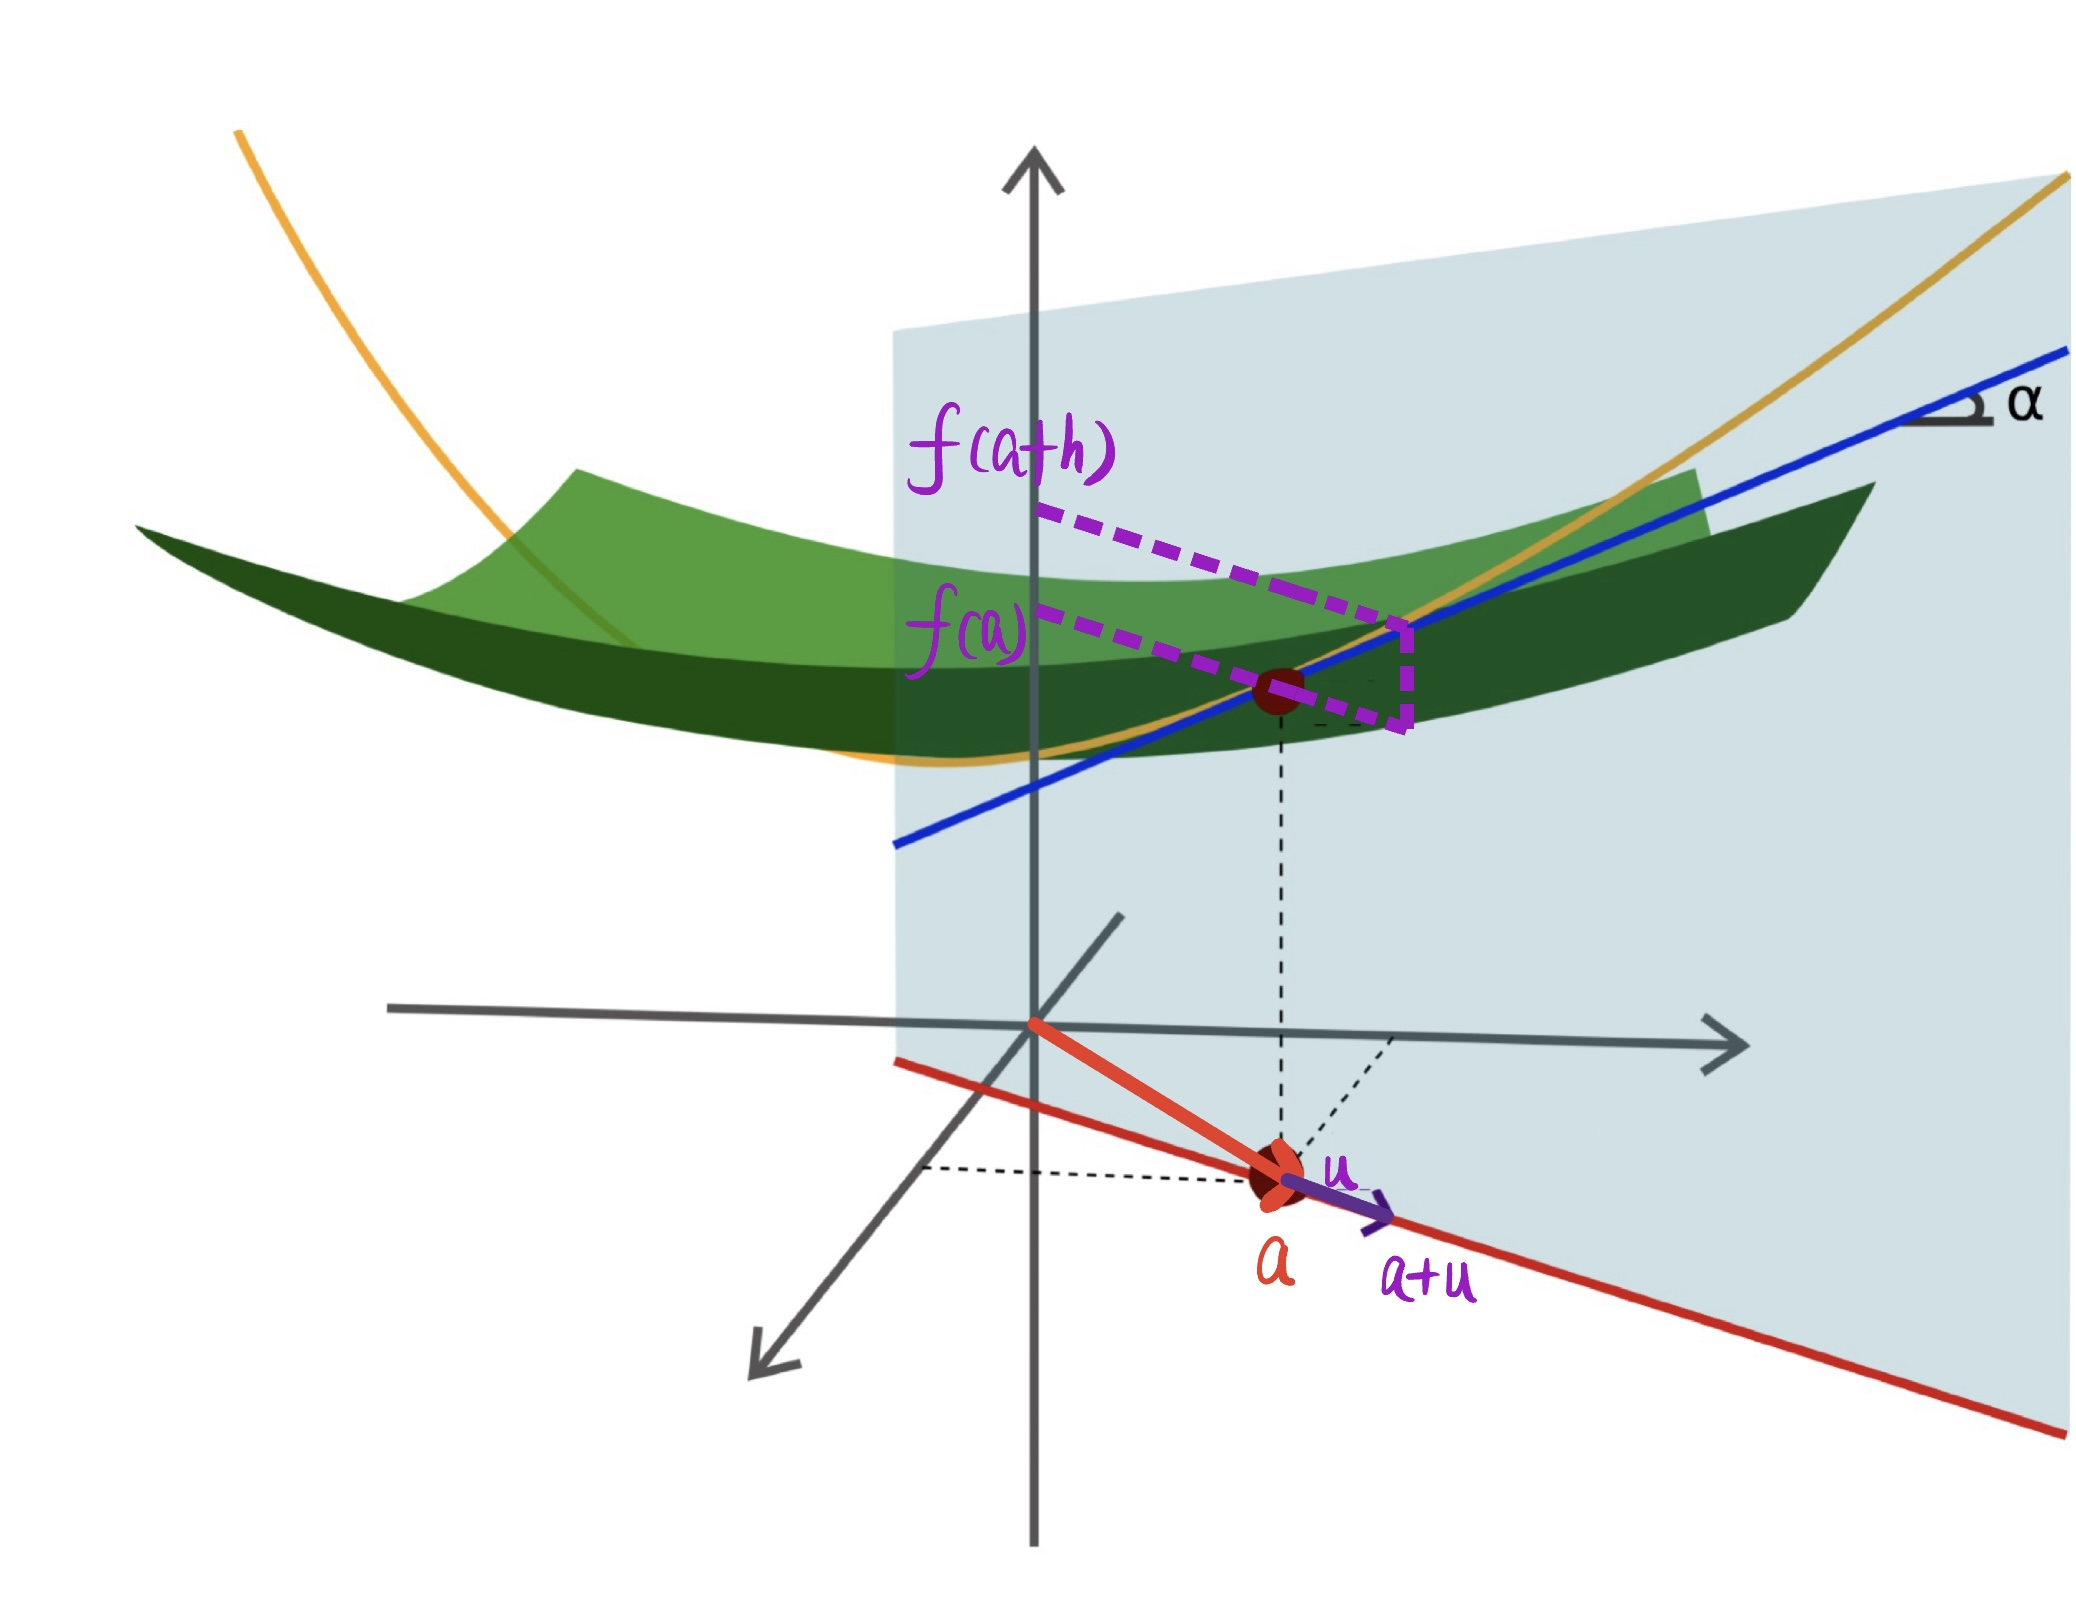
\includegraphics[scale=0.17]{images/IMG_0326.jpg}
    \caption{A picture description of directional derivative}
\end{figure}
\noindent \textbf{Remark}:
\begin{itemize}
    \item For $f:A \subset \R^2 \longrightarrow \R$, the directional derivative of the point $a$ given the unit vector $u$ is described in the picture. 
    Essentially, we are focusing on the plane in which the point $a$ and the unit vector $u$ are located. The set $f(A)$ on the plane is just a curve, if we think the unit vector $u$ as the unit vector for the $x$-axis on our new plane, then we can calculate the line tangent to $(a,f(a))$ as usual.
    \item But our purpose is to find a linear approximation near the point $a$, if we just use the directional derivative, then the linear approximation we get is the line tangent to $(a,f(a))$ on the plane, this is clerly not enough. Intuitively, for $f:A \subset \R^2 \longrightarrow \R$, 
    the best linear approximation near a point $a\in A$ should be a plane tangent to $(a,f(a))$ instead of a line.
    So assume $L:\R^2 \longrightarrow \R$ is the best linear approximation for the function $f$, we must have $$L(a+h)=f(a)+B\cdot h$$
    $B$ must be a map from $\R^2$ to $\R$, hence it should be a 1 by 2 matrix.
\end{itemize}

\noindent \textbf{Example}:
\begin{itemize}
    \item As we are familiar with all concepts of differentiation and integration of functions from $\R$ and $\R^2$ to $\R$ in high school physics. Let us consider a fuction $f:\R^2 \longrightarrow \R^2$ defined as 
    \begin{align}
        f(\begin{bmatrix}
               x \\
               y \\
        \end{bmatrix}) = 
        \begin{bmatrix}
            x+sin(y) \\
            y+sin(x) \\
        \end{bmatrix}
    \end{align}
    If we use grids to visualize the transformation $f$, we can see clearly that $f$ is not linear. But this function has a nice property, which we called \underline{locally linear}.
    If we zoom in on a given point, we can see this looks a lot more like a linear function. And the more we zoom in, the more it looks precisely like a linear function.
    \begin{figure}[ht]
        \centering
        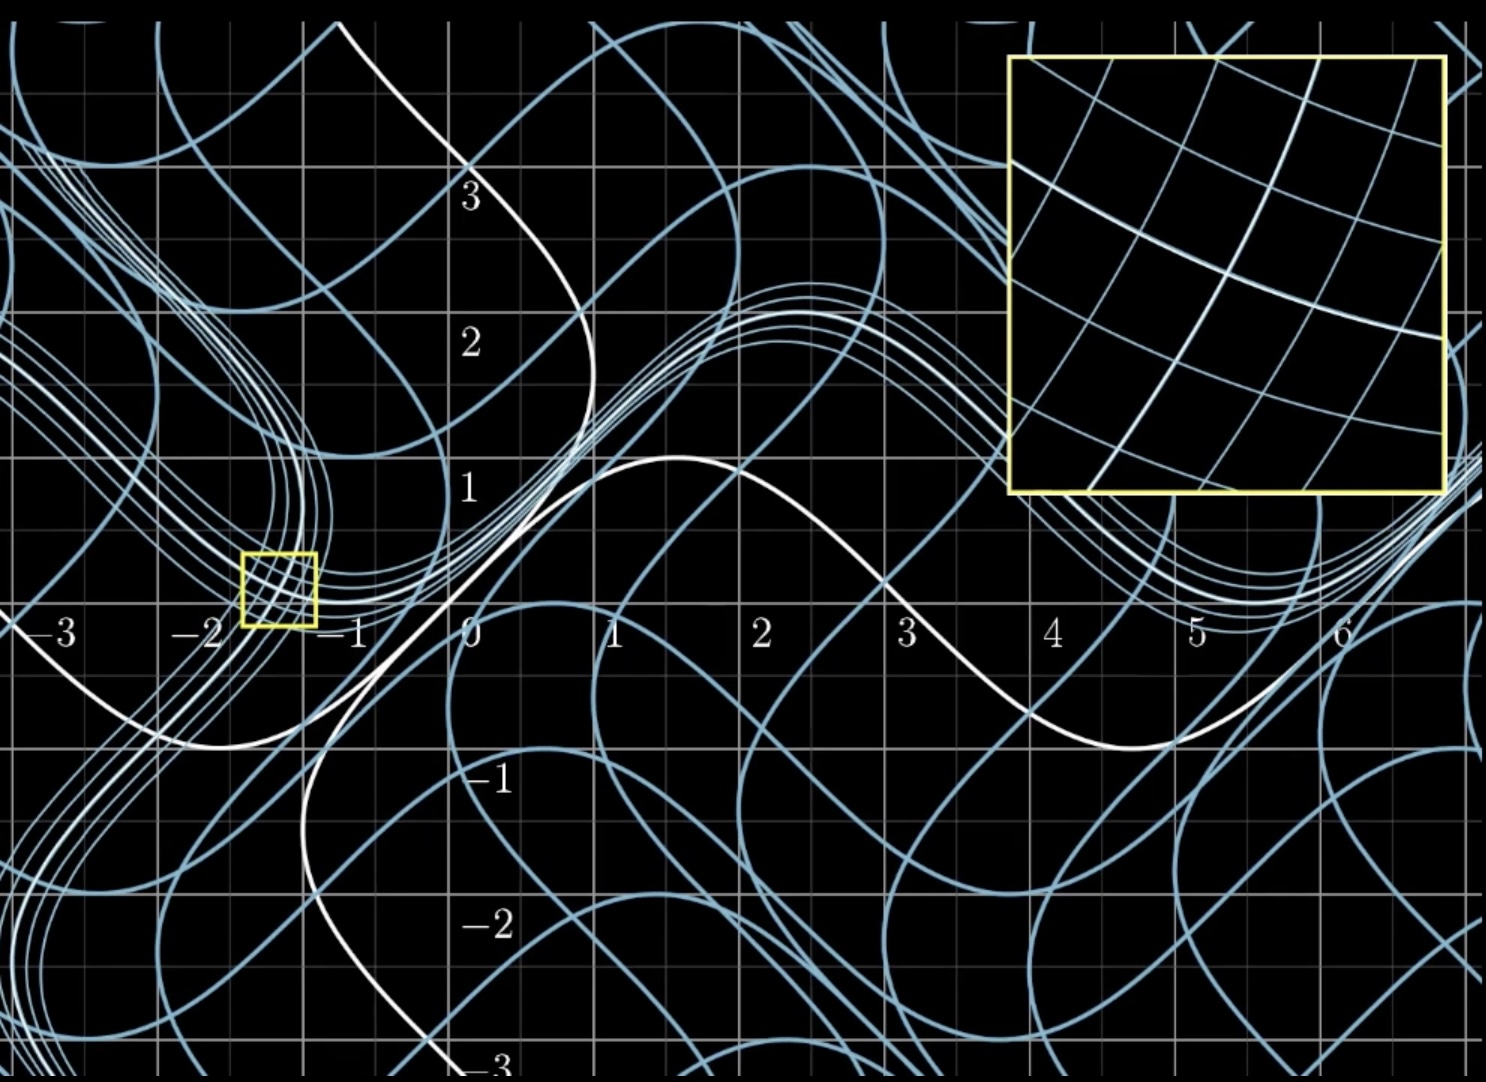
\includegraphics[scale=0.4]{images/locallylinear.jpg}
        \caption{Zoom in on a given point}
    \end{figure}
    So it is our desire to make the linear approximation on the given point $a$. Still, let $L:\R^2\longrightarrow \R^2$ be the best linear approximation, we must have 
    $$L(a+h)=f(a)+B\cdot h$$
    where $B$ should be the 2 by 2 matrix represent the linear transformation that the complicated function $f$ looks like around the point $a$.
\end{itemize}


\begin{definition}
    Let $f:A \subset \R^m \longrightarrow \R^n$. Suppose $A$ contains a neighborhood of $a$. We say that $f$ is \underline{differentiable at $a$} if there is an n by m matrix $B$ such that
    $$\lim_{\lVert h \rVert \to 0}\frac{\lVert f(a+h)-f(a)-B\cdot h \rVert}{\lVert h \rVert}=0$$
    The matrix $B$, which is unique, is called the \underline{(total) derivative} or the \underline{jacobian matrix} of $f$ at $a$, denoted as $Df(a)$.
\end{definition}

\begin{theorem}[Equivalent definition of the derivative]
    Let $f:A \subset \R^m \longrightarrow \R^n$. Suppose $A$ contains a neighborhood of $a$, if there is an n by m matrix $B$ such that
    $$\forall u \in \R^m. \lVert u \rVert =1 \Longrightarrow \lim_{t \to 0}(\frac{f(a+tu)-f(a)}{t}-B\cdot u)=0$$
    then the matrix $B$ is the derivative of $f$ at $a$.
\end{theorem}

\begin{theorem}[Uniqueness of the jacobian matrix]
    Suppose the matrix $B$ and the matrix $\tilde{B}$ both satisfy the equation above, then $B=\tilde{B}$.
\end{theorem}


\begin{theorem}
    Let $f:A\subset\R^m\longrightarrow\R^n$, if $f$ is differentiable at $a$, then $f$ is continuous at $a$.
\end{theorem}

\begin{theorem} \label{directional derivative from jmatrix}
    If the function $f:A \subset \R^m \longrightarrow \R^n$ is differentiable at the point $a$, then all the directional derivatives of $f$ at $a$ exist and $$D_uf(a)=B\cdot u$$
\end{theorem}
\noindent \textbf{Remark}:
\begin{itemize}
    \item The directional derivatives are uniquely calculated when $u \in \{e_1,\cdots,e_m\}$.
    \item However, the existence of all the directional derivatives does not guarantee that a function is differentiable at a point. For example,
    \begin{equation}
        f(x,y)=
        \begin{cases}
            \frac{x^2y}{x^4+y^2}& \text{ if } (x,y)\neq \vec{0}\\
            0& \text{ if otherwise}
        \end{cases}
    \end{equation}
    \begin{figure}[ht]
        \centering
        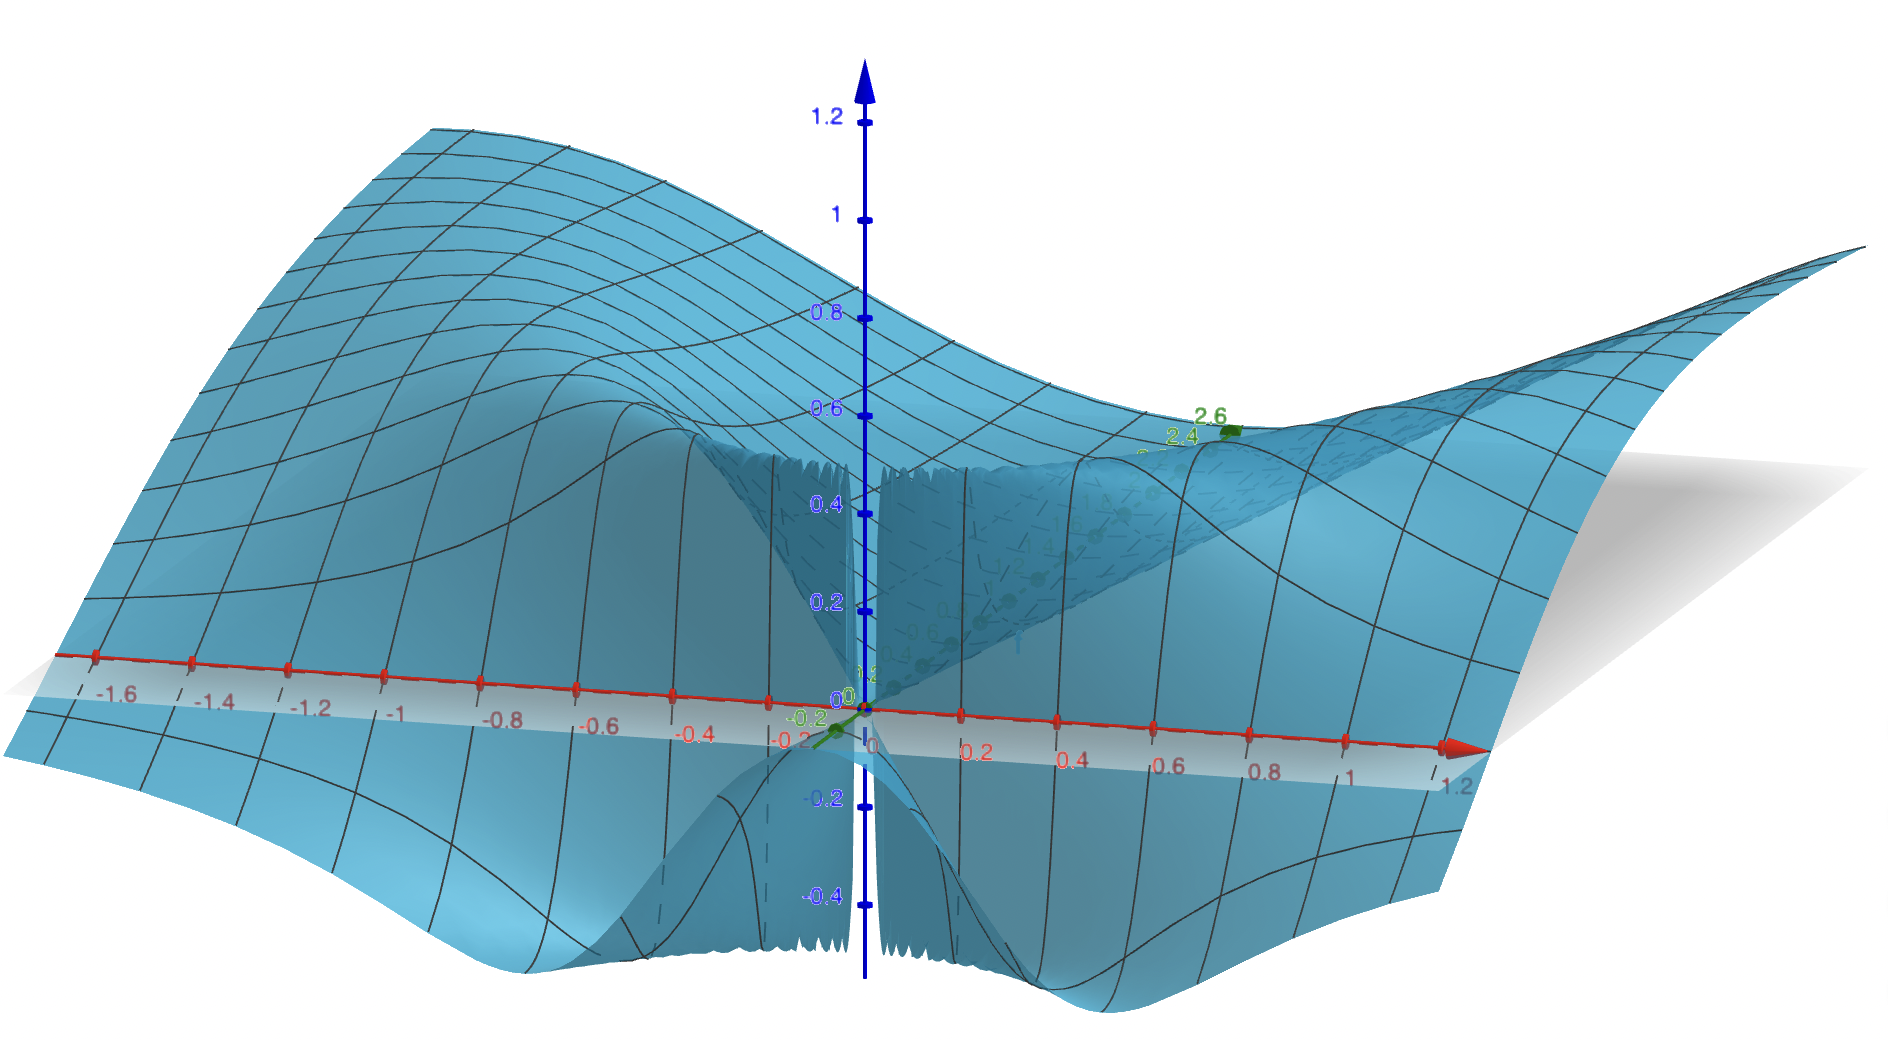
\includegraphics[scale=0.3]{images/Screen Shot 2022-09-29 at 11.44.44.png}
        \caption{$f(x,y)=\frac{x^2y}{x^4+y^2} \text{ if } (x,y)\neq \vec{0}$}
    \end{figure}
    $f$ is not differentiable at $(0, 0)$, but all of the directional derivatives exist at this point.\\
    Let $u=(h,k)\neq \vec{0}$, then
    \begin{equation}
        \begin{split}
            \frac{f(0+tu)-f(0)}{t} &= \frac{f(tu)}{t}\\
            &= \frac{(th)^2(tk)}{(th)^4+(tk)^2}\cdot \frac{1}{t}\\
            &= \frac{h^2k}{t^2h^4+k^2}
        \end{split}
    \end{equation}
    Taking the limit we have
    \begin{equation}
        \begin{split}
            D_uf(0)=\lim_{t\to 0}\frac{f(0+tu)-f(0)}{t} = \lim_{t\to 0}\frac{h^2k}{t^2h^4+k^2}
            &= \begin{cases}
                0\text{ }k=0\\
                \frac{h^2}{k}\text{ }k\neq0
            \end{cases}
        \end{split}
    \end{equation}
    We can see clearly that all directional derivatives around point 0 exist.\\
    Now we assume that $f:\R^2\longrightarrow \R$ is differentiable at $\vec{0}$. Then for some $a,b\in \R$
    $$Df(0)=\begin{bmatrix}
        a & b
    \end{bmatrix}$$
    $$Df(0)\cdot u=\begin{bmatrix}
    a & b
\end{bmatrix}\cdot u=ah+bk=D_uf(0)$$
This is a contradiction because we showed that $D_uf(0)$ is not linear.
\end{itemize}

\begin{definition}
    Let $f:A \subset \R^m \longrightarrow \R$ and $\{e_1,\cdots,e_m\}$ be the basis of $\R^m$, we define the \underline{j-th partial derivative} of $f$ at $a$ to be the directional derivative of $f$ at $a$ with respect to the vector $e_j$.
    $$D_jf(a):=D_{e_j}f(a)=\lim_{t \to 0}\frac{f(a+te_j)-f(a)}{t}$$
\end{definition}

\begin{lemma}\label{lemmajmatrix}
    Let $f:A \subset \R^m \longrightarrow \R$ be a function differentiable at $a$ and $\{e_1,\cdots,e_m\}$ be the basis of $\R^m$, then
    $$Df(a)=[D_1f(a)\cdots D_mf(a)]$$
\end{lemma}

\noindent \textbf{Example}:
\begin{itemize}
    \item Consider the function $f:\R^2\longrightarrow\R$, it can be presented as a 3-d picture.
    \begin{figure}[ht]
        \centering
        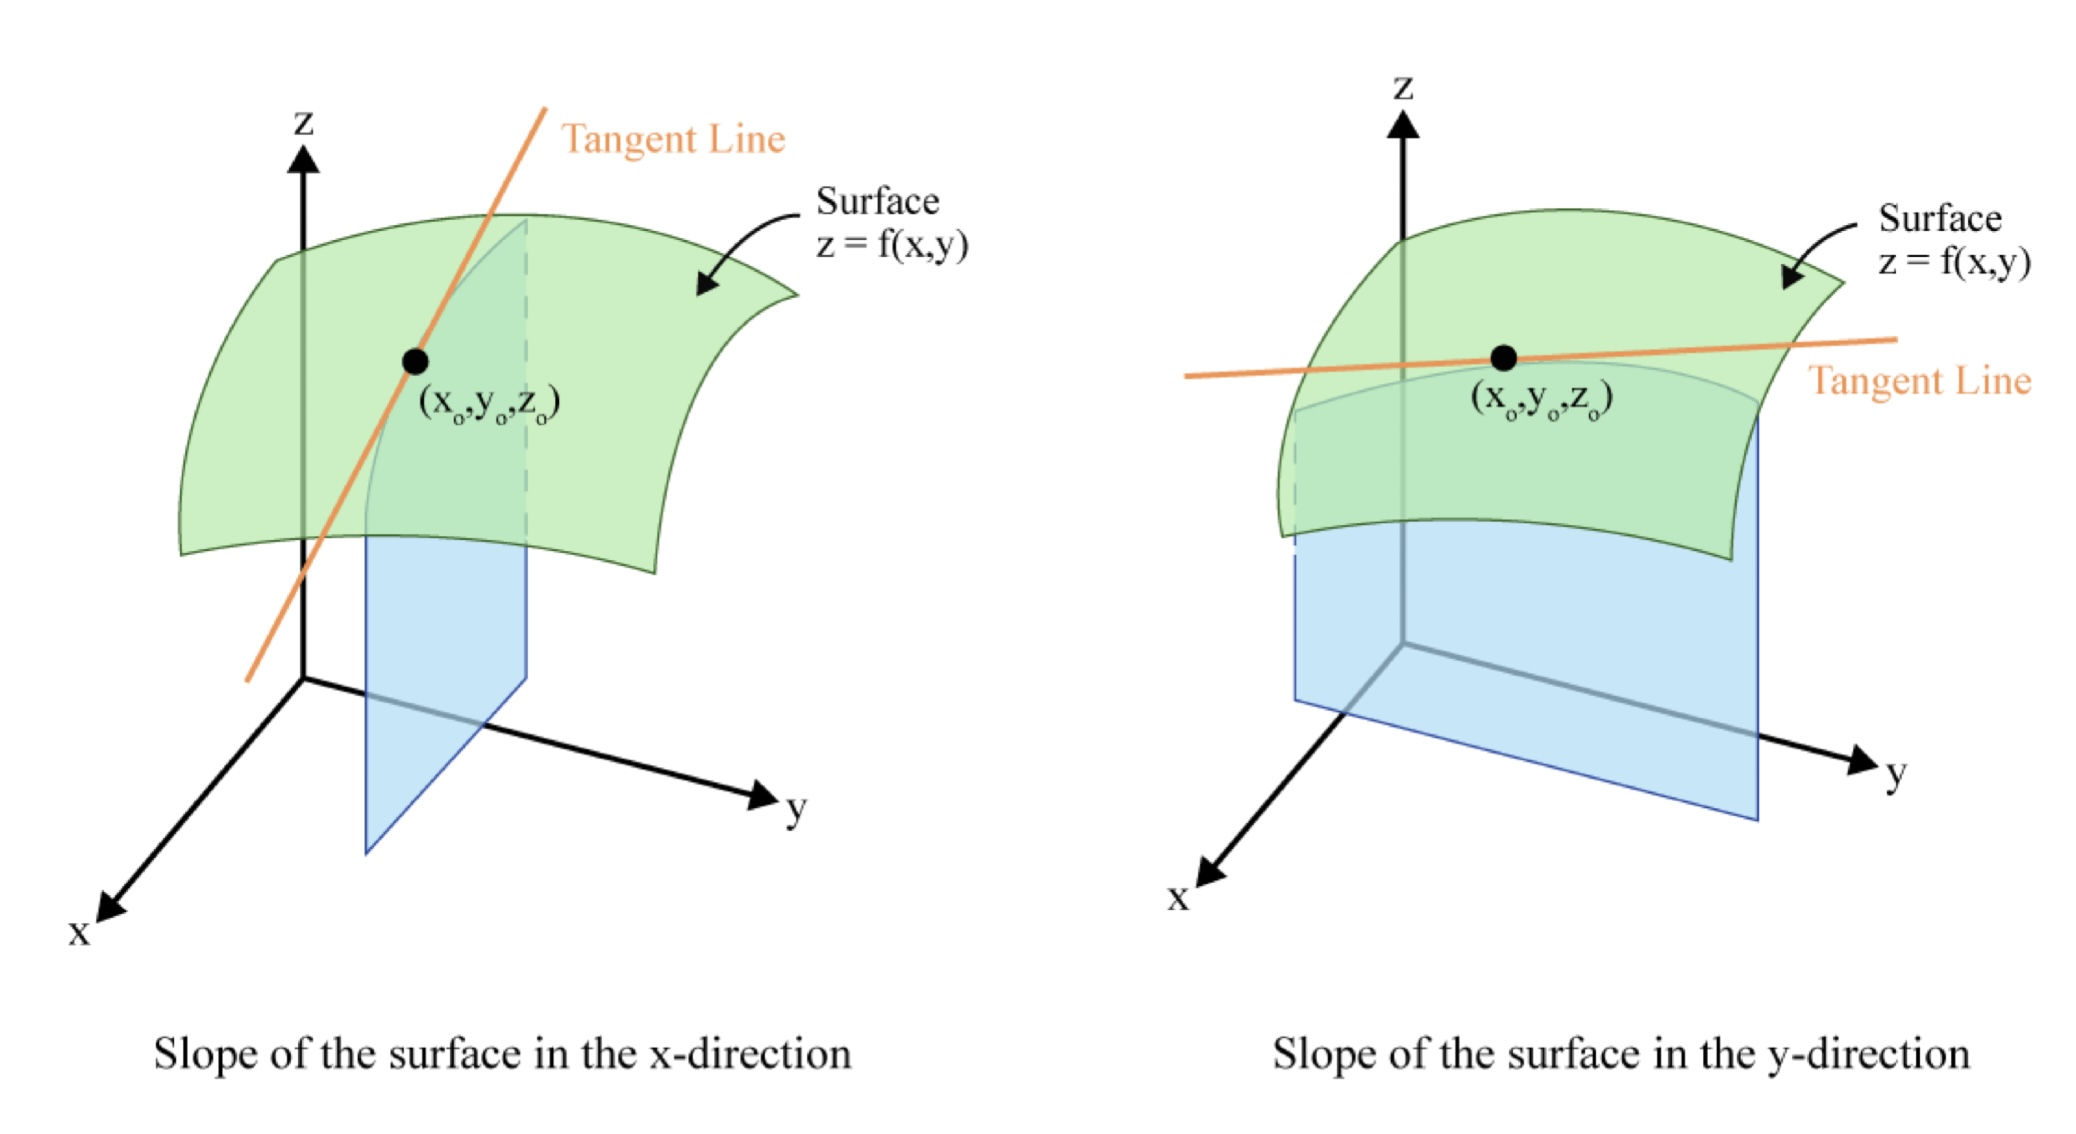
\includegraphics[scale=0.2]{images/IMG_0320.jpg}
        \caption{Partial derivative of $f:\R^2\longrightarrow \R$}
    \end{figure}
    \item Consider the function $f:\R^3\longrightarrow \R$. For $x\in \R^3$, the derivative is the row matrix
    $$Df(x)=\begin{bmatrix}
        D_1f(x)&D_2f(x)&D_3f(x)
    \end{bmatrix}$$
    In MAT240, we learnt that $Df(x)\in \mathcal{L}(\R^3,\R)$ and $\mathcal{L}(\R^3,\R)$ is a vector space of dimension $3$
    $$Df(x)=D_1f(x)\begin{bmatrix}
        1&0&0
    \end{bmatrix}+D_2f(x)\begin{bmatrix}
        0&1&0
    \end{bmatrix}+D_3f(x)\begin{bmatrix}
        0&0&1
    \end{bmatrix}$$
    Define the \underline{gradient} of $f$:
    $$\nabla f(x)=D_1f(x)e_1+D_2f(x)e_2+D_3f(x)e_3$$
    Now $\nabla f(x)$ is a vector in $\R^3$. And intuitively, \underline{it tells us the direction of the steepest increase of $x$}.
    \begin{figure}[ht]
        \centering
        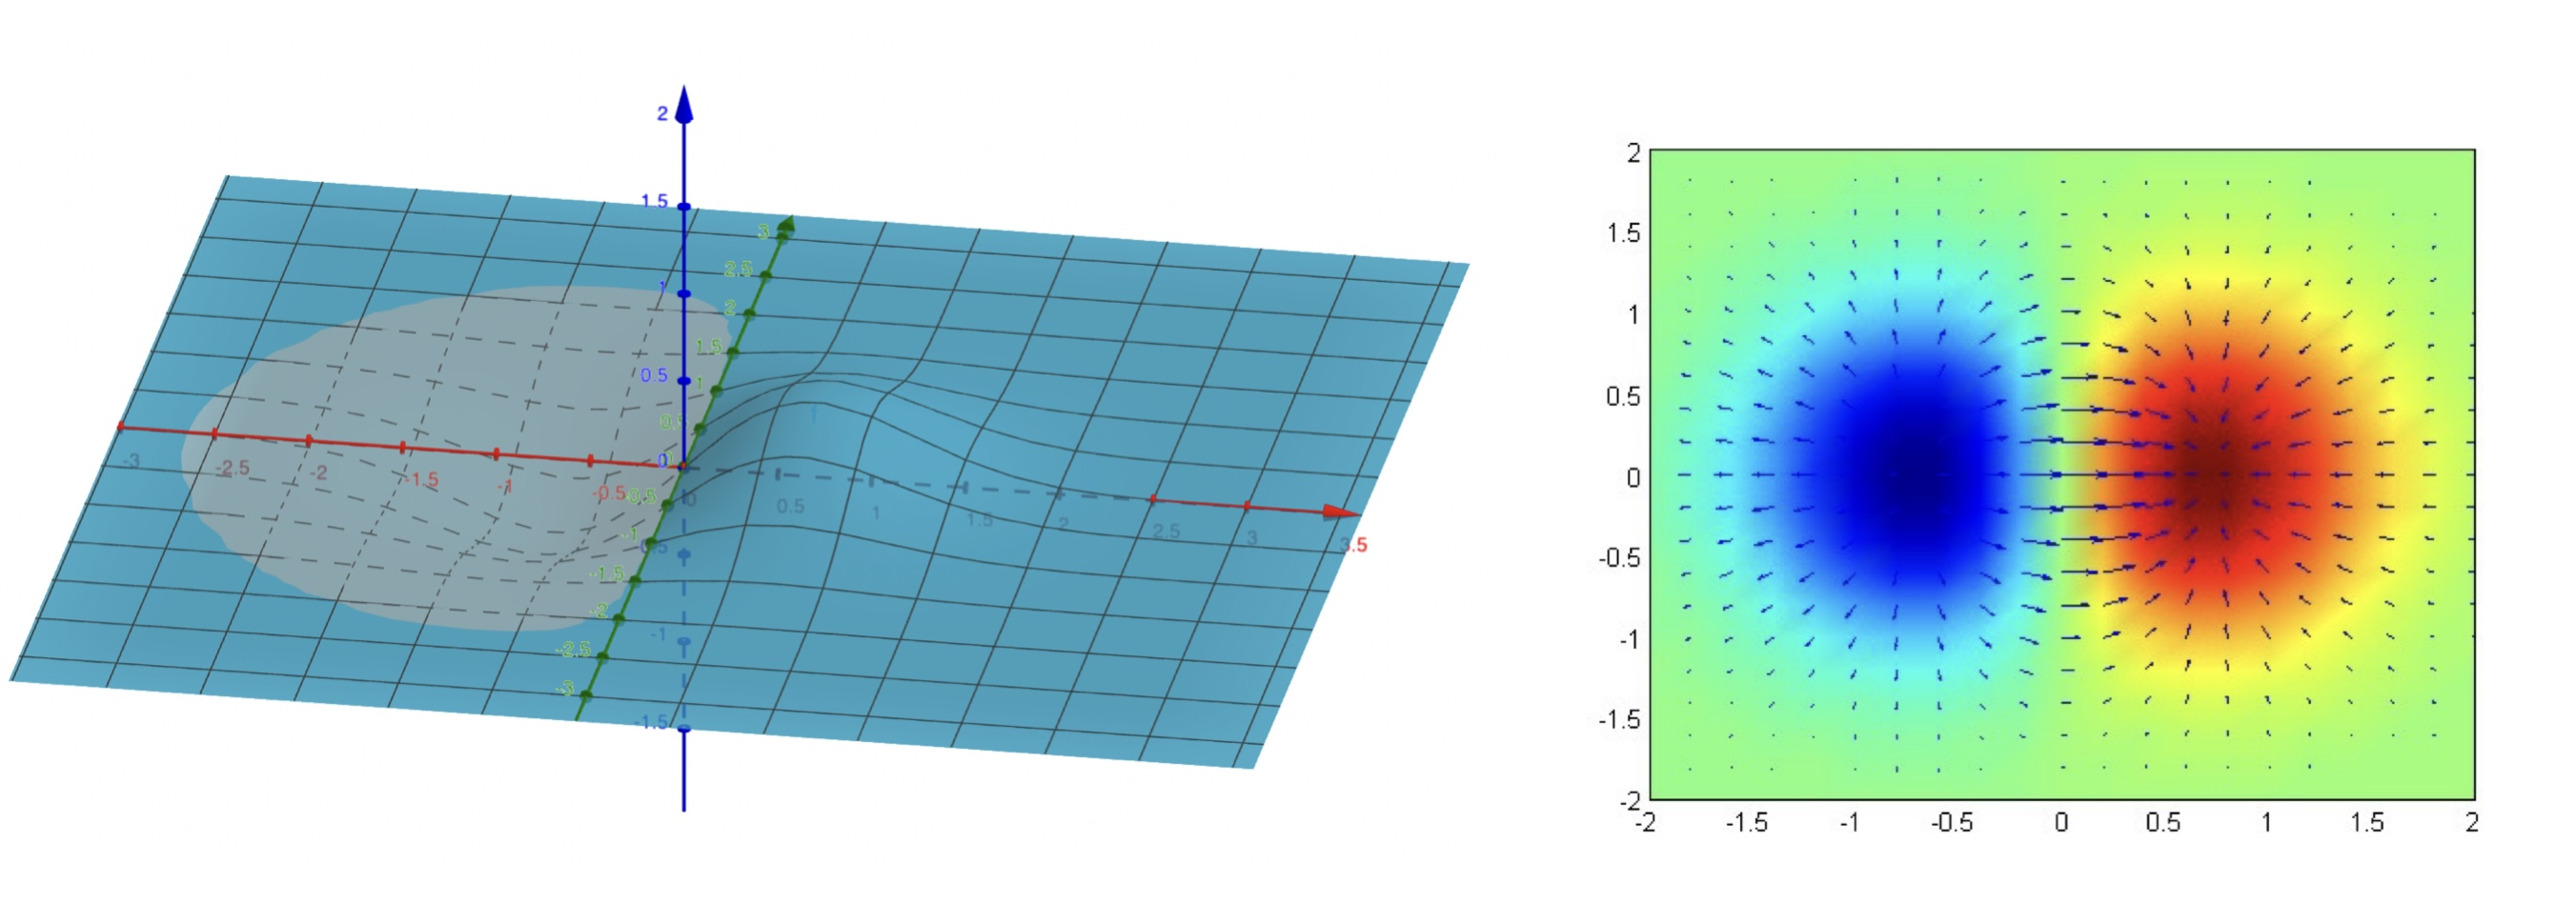
\includegraphics[scale=0.15]{images/IMG_0327.jpg}
        \caption{the gradient of $f(x,y)=xe^{-(x^2+y^2)}$}
    \end{figure}
\end{itemize}


\begin{definition}
    Let $f:A \subset \R^m \longrightarrow \R^n$, let $f_i:A\subset \R^m \longrightarrow \R$ be the \underline{i-th component function of $f$} such that
    \begin{align}
        f(a)=\begin{bmatrix}
            f_1(a)\\
            \vdots\\
            f_n(a)
        \end{bmatrix}
    \end{align}
\end{definition}

\begin{theorem} \label{differentiable iff components differentiable}
    The function $f$ is differentiable at $a$ if and only if each component function $f_i$ is differentiable at $a$.
\end{theorem}

\begin{theorem*} \label{continuous iff components continuous}
    The function $f$ is continuous at $a$ if and only if each component function $f_i$ is continuous at $a$.
\end{theorem*}

\begin{corollary}\label{lemmacompjmatrix}
    \begin{align}
        Df(a)=\begin{bmatrix}
            Df_1(a)\\
            \vdots\\
            Df_n(a)
        \end{bmatrix}
    \end{align}
\end{corollary}

\noindent \textbf{Example}:
\begin{itemize}
    \item If $f:A\subset\R\longrightarrow\R^3$ is differentiable on $A$, then $f$ is called \underline{parametrized-curve}.
    $$f(t)=\begin{bmatrix}
        f_1(t)\\
        f_2(t)\\
        f_3(t)
    \end{bmatrix}$$
    We can think $t\in A\subset\R$ as the time, and $f(t)\in \R^3$ as the displacement.$$f(t)=f_1(t)e_1+f_2(t)e_2+f_3(t)e_3$$
    \begin{figure}[ht]
        \centering
        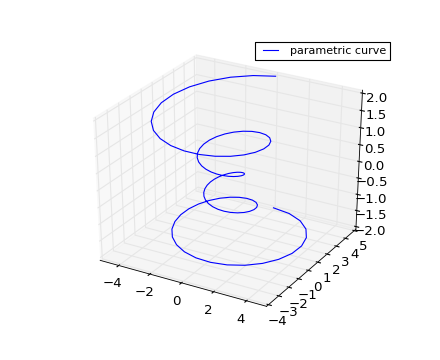
\includegraphics[scale=0.7]{images/lines3d_demo1.png}
        \caption{parametrized curve}
    \end{figure}
    By the corollary above we have
    $$Df(t)=\begin{bmatrix}
        f_1'(t)\\
        f_2'(t)\\
        f_3'(t)
    \end{bmatrix}$$
    Then the velocity vector of the curve can be represented As
    $$v(t)=f_1'(t)e_1+f_2'(t)e_2+f_3'(t)e_3$$
\end{itemize}


\begin{theorem}[Computing jacobian matrix]
    Let $f:A \subset \R^m \longrightarrow \R^n$, then 
    \begin{align}
        Df(a)=\begin{bmatrix}
            D_1f_1(a) & \cdots & D_mf_1(a)\\
            \vdots & \ddots & \vdots\\
            D_1f_n(a) & \cdots & D_mf_n(a)
        \end{bmatrix}
    \end{align}
\end{theorem}

\noindent \textbf{Example}:
\begin{itemize}
    \item Still consider the function $f:\R^2\longrightarrow \R^2$, such that 
    \begin{align}
        f(\begin{bmatrix}
               x \\
               y \\
        \end{bmatrix}) = 
        \begin{bmatrix}
            x+sin(y) \\
            y+sin(x) \\
        \end{bmatrix}
    \end{align}
    The component functions $f_1$ and $f_2$ are defined as follow:
    $$f_1:\R^2\longrightarrow\R;f_1((x,y))=x+sin(y)$$
    $$f_2:\R^2\longrightarrow\R;f_2((x,y))=y+sin(x)$$
    $f_1,f_2$ will only focus on the x-xoordinate and the y-coordinate for the vector after the transformation respectively.\\
    \begin{figure}[ht]
        \centering
        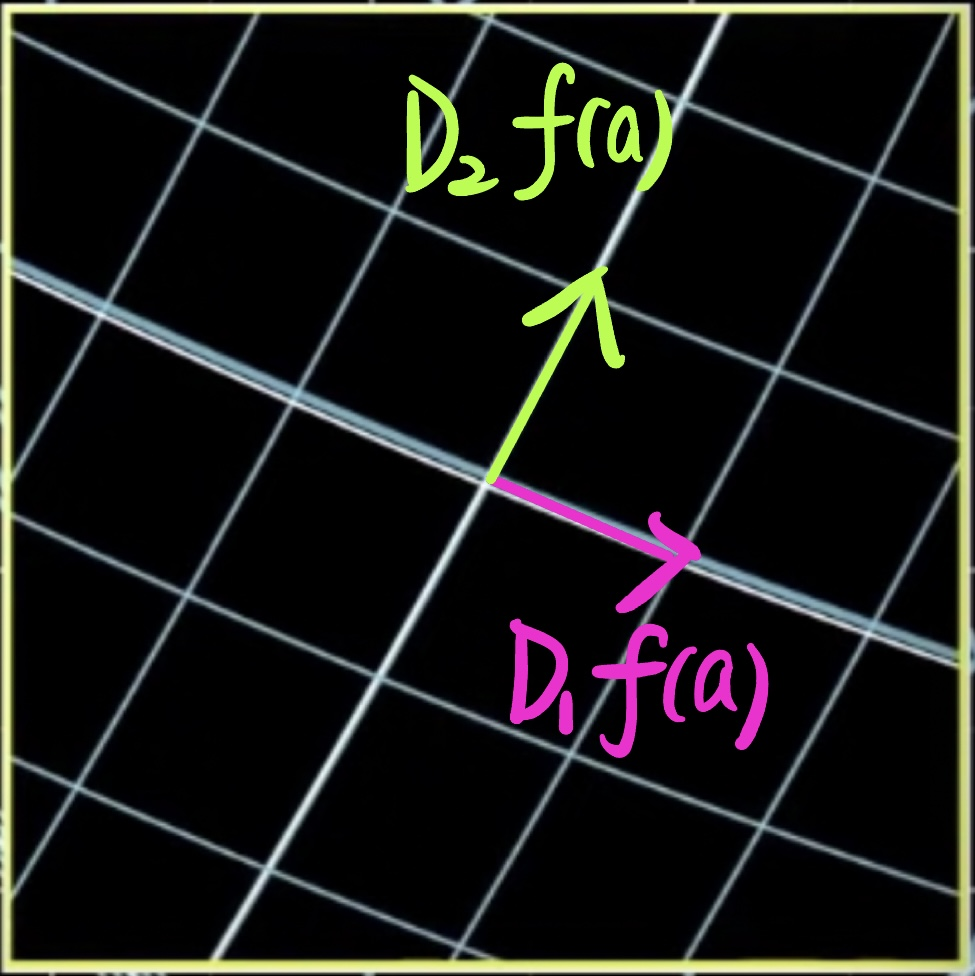
\includegraphics[scale=0.15]{images/IMG_0324.jpg}
        \caption{The place where $e_1$ and $e_2$ goes after the transformation}
    \end{figure}
    
    The matrix $B=Df(a)$ should be a 2 by 2 matrix that takes $e_1$ and $e_2$ to the corresponding spot.
    \begin{align}
        B=Df(a)=\begin{bmatrix}
            a_{1,1} & a_{1,2}\\
            a_{2,1} & a_{2,2}
        \end{bmatrix}
    \end{align}
    The vector $(a_{1,1},a_{2,1}),(a_{1,2},a_{2,2})$ is the coordinates for $D_1f(a),D_2f(a)$ respectively.\\
    If we only focus on the x-coordinates(only focus $f_1$), the first row $[a_{1,1},a_{1,2}]$ is the coordinate for $e_1,e_2$ after the transformation $f_1$.
    $$[a_{1,1},a_{1,2}]=Df_1(a)=[D_1f_1(a),D_2f_1(a)]$$
    Similarly for the second row 
    $$[a_{2,1},a_{2,2}]=Df_2(a)=[D_1f_2(a),D_2f_2(a)]$$
\end{itemize}

\section{Differentiability Classes}

\noindent \textbf{Recall}:
\begin{itemize}
    \item In single variable calculus, we can view the derivative of $f$ as a function $f':A\subset\R\longrightarrow\R$.
    It is trivial that the following statement is true.
    $$f'\text{ is continuous at }a\in A \Longrightarrow f\text{ is differentiable at } a\in A$$
    But the inverse is not true. For a very classic example
    \begin{equation}
        f(x)=
        \begin{cases}
            x^2sin(\frac{1}{x})& \text{ if }x\neq 0\\
            0& \text{ if }x=0
        \end{cases}
    \end{equation}
    \item For $f:\R\longrightarrow\R$ we defined the differentiablility classes
    \begin{itemize}
        \item $C^0$: zeroth derivative is continuous (curves are continuous).
        \item $C^1$: zeroth and first derivatives are continuous.
        \item $C^2$: zeroth, first and second derivatives are continuous.
        \item $C^k$: 0-th through k-th derivatives are continuous.
    \end{itemize}
    \item What we want is generalizing the differentiablility classes in multivariable calculus.
\end{itemize}


\begin{lemma}[Mean-Value Theorem]\label{mvt}
    If $\phi:[a,b]\longrightarrow \R$ is continuous at each point of the closed interval $[a, b]$, and differentiable at each point of the open interval $(a, b)$, then there exists a point $c \in (a, b)$ such that
    $$\phi'(c)=\frac{\phi(a)-\phi(b)}{a-b}$$
\end{lemma}


\begin{theorem} \label{continuously differentiable}
    Let $A$ be open in $\R^m$ and $f:A\subset \R^m \longrightarrow \R^n$.
    If the partial derivatives $D_jf_i(x)$ of the component functions of $f$ exist at each point $x\in A$ and are continuous on $A$.
    Then $f$ is differentiable at every $x\in A$.
\end{theorem}


\begin{definition}
    Let $A$ be open in $\R^m$ and $f:A\subset \R^m \longrightarrow \R^n$.
    \begin{itemize}
        \item $f$ is said to be \underline{of class $C^0$ on $A$}
        if $f$ is continuous on $A$.
        \item $f$ is said to be \underline{of class $C^1$ on $A$}
        if the partial derivatives $$D_jf_i(x)$$ of the component functions of $f$ exist at each point $x\in A$ and are continuous on $A$.
        \item $f$ is said to be \underline{of class $C^k$ on $A$}
        if all m-th order partial derivatives($m\leq k$) $$D_{j_1}\cdots D_{j_m}f_i$$ of the component functions of $f$ exist at each point $x\in A$ and are continuous on $A$.
        \item  $f$ is said to be \underline{of class $C^{\infty}$ on $A$} 
        if the partial derivatives of $f_i$ of all orders exist at each point $x\in A$ and are continuous on $A$
    \end{itemize}
\end{definition}
\noindent \textbf{Remark}:
\begin{itemize}
    \item Specifically, if $f$ is of class $C^1$, we say that $f$ is \underline{continuously differentiable on $A$}.
    \item We can use theorem\ref{continuously differentiable} to show that $$C^{\infty}\subset \cdots \subset C^2 \subset C^1 \subset C^0$$
\end{itemize}

\begin{theorem}
    Let $A\subset \R^m$ be open. Suppose $f:A\subset \R^m \longrightarrow\R^n$ be of class $C^2$, \\
    then $\forall i \in \{1,\cdots,n\}.\forall a \in A$ we have the relation
    $$\forall k,j \in \{1,\cdots,m\}.D_kD_jf_i(a)=D_jD_kf_i(a)$$
\end{theorem}
\noindent \textbf{Remark}:
\begin{itemize}
    \item Before trying to prove this theorem, let us get some intuition.
    Let $$f:A\subset\R^2\longrightarrow \R$$
    Consider an arbitrary $x=(a,b)\in A$, and let $h,k$ be very small.
    \begin{figure}[ht]
        \centering
        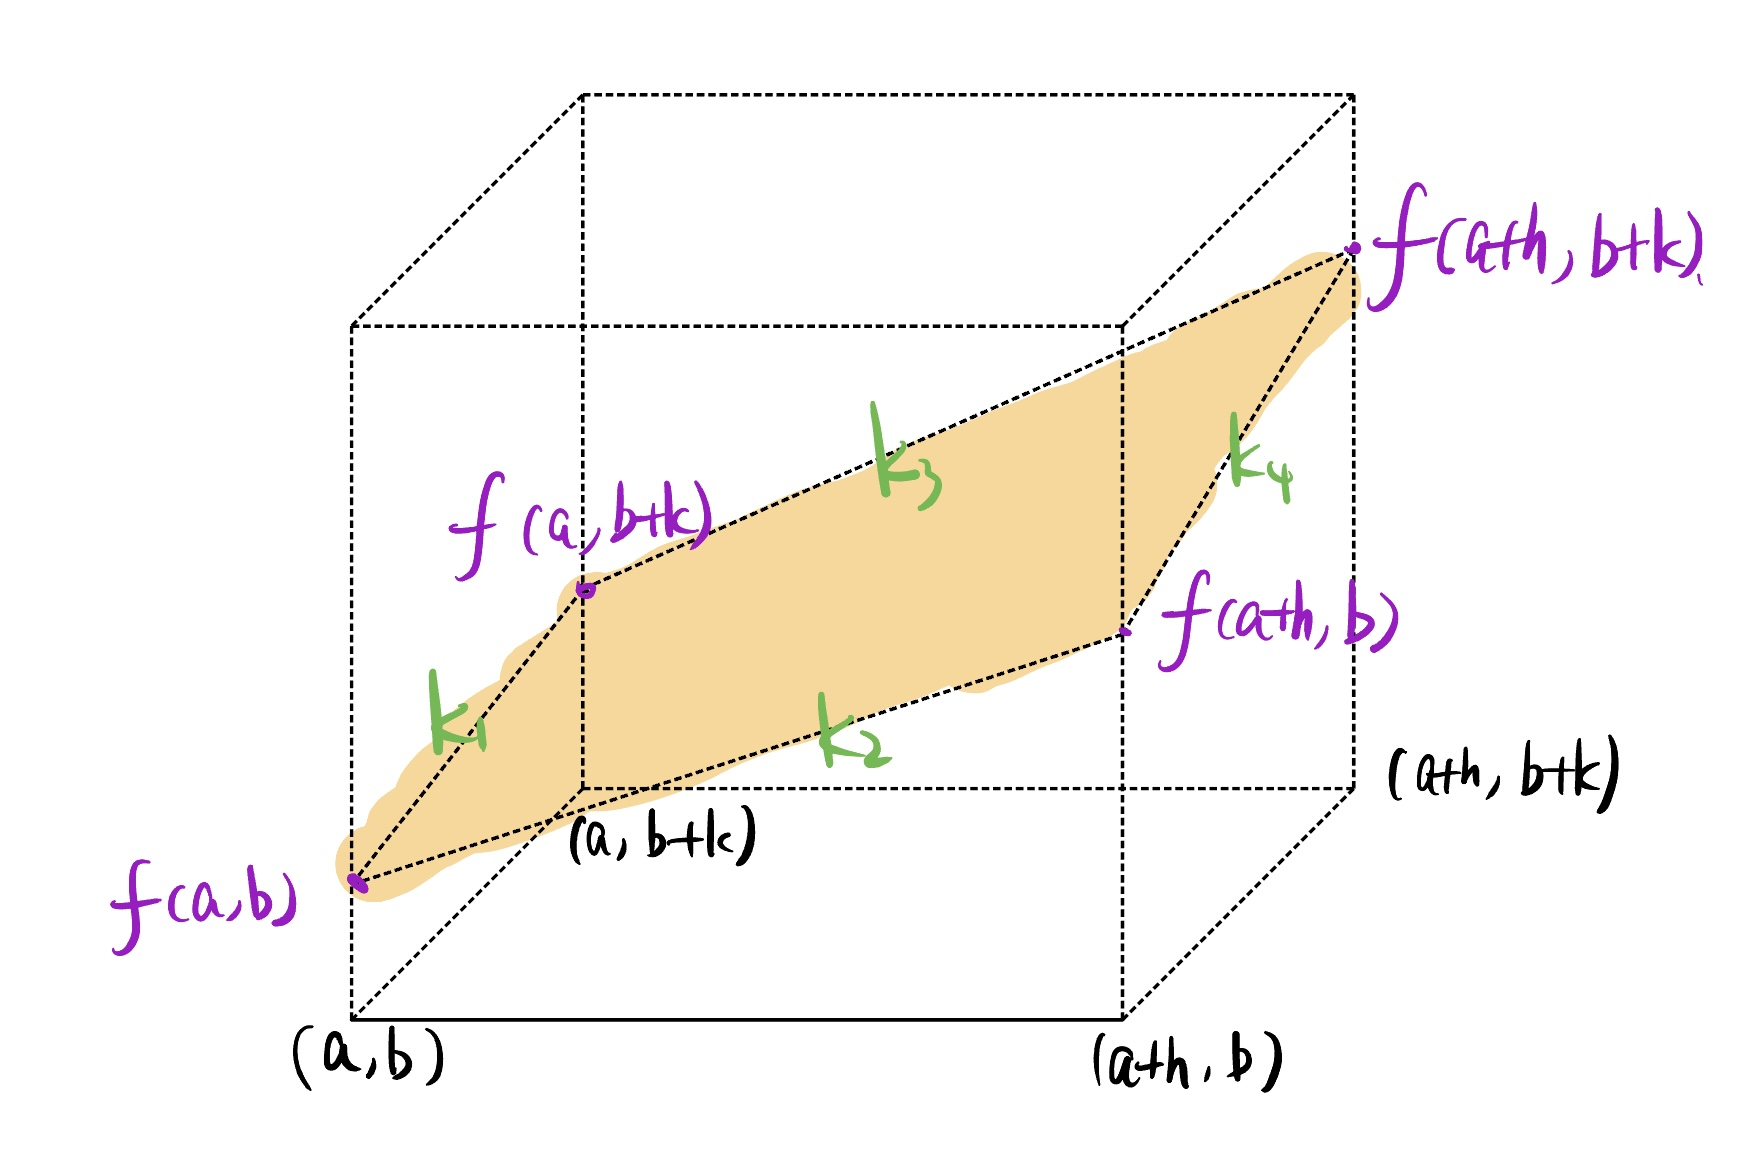
\includegraphics[scale=0.17]{images/IMG_0329.jpg}
        \caption{Geometric intuition}
    \end{figure}
    
    $Df(x)$ is the $1\times2$ matrix that represent the tangent plane at $x$.(yellow part)\\
    $D_1f(x)$ will give us the slope of the tangent line at $x$ in $e_1$ direction. For example, $$D_1f(a,b)=k_2$$
    For any point in $A\subset\R^2$, it has a corresponding slope. So 
    $$D_1f:\R^2 \longrightarrow \R$$
    By assumption, all it's partials $D_1D_1f,D_2D_1f$ are differentiable.
    \begin{equation}
        \begin{split}
            &D_2D_1f(a,b)\\
            =& \frac{k_3-k_2}{k}\\
            =& \frac{\frac{f(a+h,b+k)-f(a,b+k)}{h}-\frac{f(a+h,b)-f(a,b)}{h}}{k}\\
            =& \frac{f(a+h,b+k)-f(a,b+k)-f(a+h,b)+f(a,b)}{hk}
        \end{split}
    \end{equation}
    Similarly
    \begin{equation}
        \begin{split}
            &D_1D_2f(a,b)\\
            =& \frac{k_4-k_1}{h}\\
            =& \frac{\frac{f(a+h,b+k)-f(a+h,b)}{k}-\frac{f(a,b+k)-f(a,b)}{k}}{h}\\
            =& \frac{f(a+h,b+k)-f(a+h,b)-f(a,b+k)+f(a,b)}{hk}
        \end{split}
    \end{equation}
    So $D_2D_1f(a,b)=D_1D_2f(a,b)$. After understanding what does this theorem mean, we can formally prove it.
\end{itemize}


\begin{definition}
    Let $\vec{x}\in \R^n$, A quotient of two polynomials in multiple variables $P(\overrightarrow{x})$ and $Q(\overrightarrow{x})$
    $$R(\overrightarrow{x})=\frac{P(\overrightarrow{x})}{Q(\overrightarrow{x})}$$
    is called a \underline{rational function}, or sometimes a rational polynomial function.
\end{definition}

\begin{theorem*}\label{rational functions C_infinity}
    Let $A$ be open in $\R^m$ and let $R:A\longrightarrow \R$ be rational, then $R$ is of class $C^{\infty}$.
\end{theorem*}

\section{The Chain Rule}

\begin{definition}
    Since a matrix $A$ can be viewed as a vector, then we can define the \underline{matrix norm} of $A$, denoted as $\norm{A}$.
    satisfying the following properties:
    \begin{itemize}
        \item $\norm{A} \geq 0$ and $\norm{A}=0$ if and only if $A=0$.
        \item $\norm{\lambda A}=|\lambda|\cdot \norm{A}$ for any scaler $\lambda$.
        \item $\norm{A+B}\leq \norm{A}+\norm{B}$
    \end{itemize}
\end{definition}


\begin{definition}
    An important class of matrix norms is the \underline{subordinate matrix norms}. Given a vector norm $\norm{\cdot}$ the corresponding subordinate matrix norm is defined by
    $$\norm{A}=\sup_{x \neq 0}\frac{\norm{Ax}}{x}$$
    Or equivalently, $$\norm{A}=\sup_{\norm{x} = 1}\norm{Ax}$$
\end{definition}

\begin{lemma}\label{matrixnorm}
    A subordinate matrix norm satisfies the following properties.
    \begin{enumerate}
        \item For any vector $x$ and for any matrix $A$ $$\norm{Ax}\leq \norm{A}\cdot \norm{x}$$
        \item For ant two matrices $A$ and $B$ $$\norm{AB}\leq \norm{A}\cdot \norm{B}$$
    \end{enumerate}
\end{lemma}


\begin{definition}
    Let $A\in \mathcal{L}(\R^m,\R^n)$ be a n by m matrix. Define the \underline{ Frobenius norm}:
    $$\norm{A}_F=(\sum_{i=1}^n \sum_{j=1}^m|a_{i,j}|^2)^{\frac{1}{1}}$$
\end{definition}

\begin{theorem*}\label{all matrix norm equivalent}
    All matrix norms are equivalent.
\end{theorem*}
\noindent \textbf{Remark}:
\begin{itemize}
    \item For any $A,B\in \mathcal{L}(\R^m,\R^n)$, we define the distance function
    $$d_F(A,B)=\norm{A-B}_F$$
    This turn $\mathcal{L}(\R^m,\R^n)$ into a metric space $(\mathcal{L}(\R^m,\R^n),d_F)$.
    \item In MAT240, we proved that $\mathcal{L}(\R^m,\R^n)$ and $\R^{mn}$ are isomorphic vector spaces. It is trivial that these two metric spaces are isomorphic. $$(\mathcal{L}(\R^m,\R^n),d_F) \cong (\R^{nm},d_2)$$
    \item By theorem\ref{all matrix norm equivalent}, no matter which matrix norm we choose, it induce the same topology. So we need to take care with $(\mathcal{L}(\R^m,\R^n),d_F)$ in order to learn the structure of the topological space $\mathcal{L}(\R^m,\R^n)$.
\end{itemize}


\begin{theorem}[Chain Rule]\label{Chain Rule}
    Let $A\subset \R^m$, $B\subset \R^n$. Let $f:A\subset\R^m \longrightarrow \R^n$ and $g:B\subset\R^n \longrightarrow \R^p$ with $f(A)\subset B$.
    If $f$ is differentiable at $a$ and $g$ is differentiable at $f(a)$. Then $g \circ f$ is differentiable at $a$, furthermore $$D(g\circ f)(a)=Dg(f(a))\cdot Df(a)$$
\end{theorem}


\begin{corollary}\label{composition also in Cr}
    Let $A\subset \R^m$, $B\subset \R^n$. Let $f:A\subset\R^m \longrightarrow \R^n$ and $g:B\subset\R^n \longrightarrow \R^p$ with $f(A)\subset B$.
    If $f$ and $g$ are of class $C^r$. Then $g \circ f$ is of class $C^r$.
\end{corollary}

\begin{theorem}[MVT in multivariable]\label{MVTmultivariable}
    Let $A\subset \R^m$ be open..  Let $f:A\subset \R^m \longrightarrow \R$ be differentiable on $A$.
    If $A$ contains the line segment with end points $a$ and $b$, then there exists a point $p=a+t_0(b-a)$ in the line segment.($t_0\in(0,1)$) such that
    $$f(b)-f(a)=Df(p)(b-a)$$
\end{theorem}

\section{The Inverse Function Theorem}

\noindent \textbf{Motivation}:
\begin{itemize}
    \item Consider the system of equations 
    \begin{equation}
        \begin{cases}
            x^3-7x^2+e^x\cdot y^2+sin(y)=b_1\\
            x^4\cdot y^3-x+y=b_2
        \end{cases}
    \end{equation}
    Since it has two equations and two unknowns. 
    We can now view it as a function $f:\R^2\longrightarrow \R^2$. 
    More generaly, if we have a system of equations that has $n$ equations and $n$ unknowns, we can view it as a function $f:\R^n \longrightarrow \R^n$.
    \item Consider the easy case where $f(x)$ is linear. In other words $f(x)=Ax$ where $A$ is a fixed n by n matrix. This is now an easy linear algebra problem, if $A$ is invertible, we can find the inverse of $A$ to solve the equation. $$x=A^{-1}\cdot y_0$$
    \item Now consider a more general case, suppose $f:\R^n\longrightarrow\R^n$ is differentiable at $x_0$.  What we want is to solve $f(x)=y$ for $|y-y_0|$ very small.
    \item The non-singularity of $Df$ implies that $f$ is locally one-to-one.
\end{itemize}

\begin{theorem*}\label{TIFlemma1}
    Let $f:A \subset \R^m\longrightarrow\R^n$
    \begin{itemize}
        \item If it is differentiable, we can view its derivative as a function $$Df:\R^m\longrightarrow\mathcal{L}(\R^m,\R^n)$$
        \item If we choose the Euclidean norm $\norm{\cdot}_2$ for $\R^m,\R^n$, then we can define the matrix norm as(also works for other matrix norms) $$\norm{Df(x)}_2=\sup_{\norm{u}_2=1}\norm{Df(x)\cdot u}_2$$
    \end{itemize}
    Then we have the equivalence
    $$f\text{ is of class }C^1 \text{ on }A \Longleftrightarrow Df \text{ is continuous between metric spaces.}$$
    In other words: $f$ is of $C^1$ if and only if for any $a\in A$
    $$\forall \epsilon>0. \exists \delta>0.\forall x \in \R^m. \norm{x-a}_2<\delta \Longrightarrow \norm{Df(x)-Df(a)}_2<\epsilon$$
\end{theorem*}
\noindent \textbf{Remark}:
\begin{itemize}
    \item This is a theorem I came up with myself.
    \item This will be helpful for the next lemma for our final theorem(the inverse function theorem).
    \item If we do not specify the norm, then we just use the Euclidean norm.
    \item Theorem\ref{all matrix norm equivalent} shows that other matrix norms also work. I choose this matrix norm because we only talked about this norm in class.
    \item Actually, we can generalize this theorem further.
\end{itemize}

\begin{theorem*}\label{TIFlemma1.5}
    Let $f:A \subset \R^m\longrightarrow\R^n$
    \begin{itemize}
        \item If it is differentiable, we can view its derivative as a function $$Df:\R^m\longrightarrow\mathcal{L}(\R^m,\R^n)$$
        \item Can choose any matrix norm to turn $\mathcal{L}(\R^m.\R^n)$ into a metric space.(For convenience, we choose the Frobenius norm)
    \end{itemize}
    Then we have the equivalence for $k \geq 1$
    $$f\text{ is of class }C^k \text{ on }A \Longleftrightarrow Df \text{ is of class } C^{k-1}$$
\end{theorem*}

\begin{lemma}\label{TIFlemma2}
    Let $A$ be open in $\R^n$, let $f:A\longrightarrow\R^n$ be of class $C^1$ on $A$. 
    If $Df(a)$ is non-singular, then 
    $$\exists \epsilon>0\exists \alpha>0. \forall x_1,x_2\in B(a;\epsilon). \norm{f(x_2)-f(x_1)}\geq \alpha \norm{x_2-x_1}$$
\end{lemma}
\noindent \textbf{Remark}:
\begin{itemize}
    \item Notice that $B(a;\epsilon)\subset A$ because all $x \in B(a;\epsilon)$ is defined for $f$.
    \item This shows that $\exists \epsilon>0$ such that $f:B(a;\epsilon)\longrightarrow\R^n$ is one-to-one(injective).
    \item The term one-to-one function (injective function) must not be confused with one-to-one correspondence that refers to bijective functions
\end{itemize}

\begin{lemma}\label{extremum 0matrix}
    Let $A$ be open in $\R^n$ and $\phi:A\longrightarrow\R$. Suppose $\phi$ is differentiable on $A$ and has a local minimum(or maximum) at $x_0\in A$, then $$D\phi(x_0)=\begin{bmatrix}
        0 & \cdots & 0
    \end{bmatrix}$$
\end{lemma}


\begin{theorem}\label{TIFintermediathm}
    Let $A\subset \R^n$ be open and $f:A\longrightarrow \R^n$ be of class $C^r$ for $r \geq 1$. Let $B=f(A)$. Assume
    \begin{itemize}
        \item $f$ is one-to-one on $A$.
        \item $Df(x)$ is non-singular at all $x\in A$.
    \end{itemize}
    Then we have
    \begin{itemize}
        \item $B\in \R^n$ is open.
        \item $g=f^{-1}:B\longrightarrow A$ is also of $C^r$.
    \end{itemize}
\end{theorem}

\begin{theorem}[The Inverse Function Theorem]
    Let $A$ be open in $\R^n$ and let $f:A\longrightarrow \R^n$ be of class $C^r$. 
    If $Df$ is non-singular at the point $a\in A$.
    Then we have
    \begin{itemize}
        \item There is an open $U$ containing $a$ and an open $V\subset\R^n$ containing $f(a)$ such that $f:U\longrightarrow V$ is bijective.
        \item The inverse $g=f^{-1}:V \longrightarrow U$ is also of class $C^r$.
    \end{itemize}
\end{theorem}

\noindent \textbf{Remark}:
\begin{itemize}
    \item This is a very long and difficult theorem, but it is very important.
    \item In the future, we will generalize this theorem in terms of differentiable maps between differentiable manifolds.$$F:M\longrightarrow N$$ 
    \item If the derivative is non-singular at a point $a$, then we have a very nice result. There is a small part $U$ of $M$ containing $a$ and a small part $V$ of $N$ containing $F(a)$, such that $U$ and $V$ are isomorphic.
\end{itemize}

\section{Applications}

\subsection{Approximation}

There are four kinds of multivariable functions
\begin{itemize}
    \item Curves: $f:\R\longrightarrow \R^n$
    \item Surfaces: $f:\R^2\longrightarrow \R^n$
    \item Scaler fields: $f:\R^n \longrightarrow \R$
    \item Vector fields: $f:\R^n \longrightarrow \R^m$
\end{itemize}
In this section, we will focus on the scalar fields. For example
\begin{itemize}
    \item In physics, we often encounter fields, which is a function associating a single number to every point in a space.
    \item In machine learning and artificial intelligence, we have the cost function(sometimes also called an error function) which is a function that maps an event or values of one or more variables onto a real number intuitively representing some cost associated with the event.
\end{itemize}
Our goal is to learn the optimization for scalar field functions.\\
\begin{definition}
    We say a function $f(x_1,\cdots,x_n)$ is \underline{linear} if $$f(x_1,\cdots,x_n)=a_1x_1+\cdots+a_nx_n+c$$
\end{definition}

\begin{definition}
    A \underline{linear form} is a polynomial with terms all of degree one.
\end{definition}

\begin{definition}
    Given a differentiable function $f:\R^n\longrightarrow \R$ and a point $a\in \R^n$. The \underline{linear approximation} of $f$ at $a$ is
    $$L(x)=f(a)+Df(a)\cdot (x-a)$$
\end{definition}
\noindent \textbf{Remark}:
\begin{itemize}
    \item Let $x=(x_1,\cdots,x_n)$ and $a=(a_1,\cdots,a_n)$. Then 
    \begin{equation}
        \begin{split}
            L(x_1,\cdots,x_n)&=f(a)+Df(a)\cdot (x-a)\\
            &= f(a)+ \begin{bmatrix}
                D_1f(a) & \cdots & D_nf(a)
            \end{bmatrix}\cdot \begin{bmatrix}
                x_1-a_1\\
                \vdots\\
                x_n-a_n
            \end{bmatrix}\\
            &= f(a)+ D_1f(a)(x_1-a_1)+\cdots+D_nf(a)(x_n-a_n)\\
            &= f(a)+ \nabla f(a)\cdot (x_1-a_1,\cdots,x_n-a_n)
        \end{split}
    \end{equation}
\end{itemize}

\begin{definition}
    We say a function $f(x_1,\cdots,x_n)$ is \underline{quadratic} if $f$ is a polynomial of degree 2.
\end{definition}
\noindent \textbf{Example}:
\begin{itemize}
    \item $f(x)=ax^2+bx+c$ is a quadratic function of one variable.
    \item $f(x,y)=ax^2+by^2+cxy+dx+ey+f$ is a quadratic function of two variables.
    \item $f(x,y,z)=ax^2by^2+cz^2+dxy+exz+fyz+gx+hy+iz+j$ is a quadratic function of three variables.
\end{itemize}

\begin{definition}
    A \underline{quadratic form} is a polynomial with terms all of degree two.
\end{definition}
\noindent \textbf{example}:
\begin{itemize}
    \item $ax^2+2bxy+cy^2$ is a quadratic form. Also notice that
    \begin{equation}
        ax^2+2bxy+cy^2=\begin{bmatrix}
            x & y
        \end{bmatrix}\begin{bmatrix}
            a & b\\
            b & c
        \end{bmatrix}\begin{bmatrix}
            x\\
            y
        \end{bmatrix}
    \end{equation}
    \item $ax^2+dy^2+fz^2+2bxy+2cxz+2dyz$ is a quadratic form. Also notice that
    \begin{equation}
        ax^2+dy^2+fz^2+2bxy+2cxz+2dyz=\begin{bmatrix}
            x & y & z
        \end{bmatrix}\begin{bmatrix}
            a & b & c\\
            b & d & e\\
            c & e & f
        \end{bmatrix}\begin{bmatrix}
            x\\
            y\\
            z
        \end{bmatrix}
    \end{equation}
\end{itemize}
\noindent \textbf{Remark}:
\begin{itemize}
    \item A quadratic function $f(x_1,\cdots,x_n)$ can be witten as a sum of a linear form $l(x_1,\cdots,x_n)$ and a quadratic form $q(x_1,\cdots,x_n)$ plus a constant.
    $$f(x_1,\cdots,x_n)=c+l(x_1,\cdots,x_n)+q(x_1,\cdots,x_n)$$
    \item As $n$ getting more and more large, the quadratic form $q(x_1,\cdots,x_n)$ will getting extremly complicated. It is our desire to use an associated matrix to get the quadratic form.
\end{itemize}

\begin{definition}
    Let $f:\R^n\longrightarrow \R$ be of class $C^2$. The \underline{Hessian matrix} of $f$ at point $a$ is defined as
    $$Hf(a)=\begin{bmatrix}
        D_1D_1f(a) & \cdots & D_1D_nf(a)\\
        \vdots & \ddots & \vdots\\
        D_nD_1f(a) & \cdots & D_nD_nf(a)
    \end{bmatrix}$$
    sometimes we also use the notation $D^2f(a)$ to denote the Hessian matrix.
\end{definition}
\noindent \textbf{Remark}:
\begin{itemize}
    \item The Hessian matrix of a function $f$ at point $a$ contains all the information of all second order partial derivatives of $f$ at $a$.
    \item Consider the gradient of $f$
    $$\nabla f :\R^n \longrightarrow\R^n$$
    The Hessian matrix of $f$ is the Jacobian matrix of the gradient of $f$.
    $$Hf=D(\nabla f)$$
    \item The Hessian matrix of $f$ can also be viewed as the Jacobian matrix of the Jacobian matrix of $f$.
    $$Hf=D(D f)$$
    This is why we choose the notation $D^2f$.
\end{itemize}

\begin{definition}
    Let $f:\R^n\longrightarrow \R$ be of class $C^2$. Then the \underline{quadratic approximation} of $f$ at the point $a$ is 
    $$Q(x)=f(a)+Df(a)\cdot(x-a)+\frac{1}{2}(x-a)^TD^2f(a)(x-a)$$
\end{definition}
\noindent \textbf{Remark}:
\begin{itemize}
    \item Let $x=(x_1,\cdots,x_n)$ and $a=(a_1,\cdots,a_n)$. $(x-a)^T$ denote the transpose of the vector $(x-a)$.
    $$(x-a)^T=\begin{bmatrix}
        x_1-a_1\\
        \vdots\\
        x_n-a_n
    \end{bmatrix}^T=\begin{bmatrix}
        x_1-a_1 & \cdots & x_n-a_n
    \end{bmatrix}$$
    \item Can check that
    \begin{itemize}
        \item $Q(a)=f(a)$
        \item $D_iQ(a)=D_if(a)$ for all $i$.
        \item $D_iD_jQ(a)=D_iD_jf(a)$ for all $i,j$.
        \item All partial derivatives of order geater than or equal to three are all zero.
    \end{itemize}
    \item The quadratic approximation will be very useful in physics.
\end{itemize}
\noindent \textbf{Example}:
\begin{itemize}
    \item Let $f:\R^2 \longrightarrow \R$ be of class $C^2$. The quadratic approximation for $f$ at point $a=(a_1,a_2)$ is
    \begin{equation}
        \begin{split}
            Q(x_1,x_2)=&f(a)+D_1f(a)(x_1-a_1)+D_2f(a)(x_2-a_2)\\
            &+\frac{1}{2}D_1D_1f(a)(x_1-a_1)^2+D_1D_2f(a)(x_1-a_1)(x_2-a_2)+\frac{1}{2}D_2D_2f(a)(x_2-a_1)^2
        \end{split}
    \end{equation}
    \item Let $f(x,y)=e^{\frac{x}{2}}sin(y)$. Compute the quadratic approximation of $f$ at $(0,\frac{\pi}{2})$
    $$f(0,\frac{\pi}{2})=e^0sin(\frac{\pi}{2})=1$$
    $$D_1f(x,y)=\frac{1}{2}e^{\frac{\pi}{2}}sin(y);\quad D_1f(0,\frac{\pi}{2})=\frac{1}{2}$$
    $$D_2f(x,y)=e^{\frac{\pi}{2}}cos(y);\quad D_2f(0,\frac{\pi}{2})=0$$
    $$D_1D_1f(x,y)=\frac{1}{4}e^{\frac{\pi}{2}}cos(y);\quad D_1D_1f(0,\frac{\pi}{2})=\frac{1}{4}$$
    $$D_2D_2f(x,y)=-e^{\frac{\pi}{2}}sin(y);\quad D_2D_2f(0,\frac{\pi}{2})=-1$$
    The linear approximation of $f$ at $a$ is 
    \begin{equation}
        \begin{split}
            L(x,y)&=f(0,\frac{\pi}{2})+D_1f(0.\frac{\pi}{2})(x-0)+D_2f(0,\frac{\pi}{2})(y-\frac{\pi}{2})\\
            &=1 + \frac{1}{2}x+0\\
            &= \frac{1}{2}x+1
        \end{split}
    \end{equation}
    So the quadratic approximation is 
    \begin{equation}
        \begin{split}
            Q(x,y)&=L(x,y)+\frac{1}{2}D_1D_1f(0,\frac{\pi}{2})(x-0)^2+D_1D_2f(0,\frac{\pi}{2})(x-0)(y-\frac{\pi}{2})+\frac{1}{2}D_2D_2f(0,\frac{\pi}{2})(y-\frac{\pi}{2})^2\\
            &= L(x,y)+\frac{1}{2}x^2-\frac{1}{2}(y-\frac{\pi}{2})^2\\
            &= 1+\frac{1}{2}x+\frac{1}{2}x^2-\frac{1}{2}(y-\frac{\pi}{2})^2
        \end{split}
    \end{equation}
\end{itemize}

\subsection{Optimization(with constraints)}

\begin{definition}
    Let $f:A\subset \R^n \longrightarrow \R$ 
    \begin{enumerate}
        \item $f$ is said to have a \underline{local maxima} at the point $a\in A$ if 
        $$\exists \delta>0.\forall x \in A. \norm{x-a}<\delta\Longrightarrow f(x)\leq f(a)$$
        \item $f$ is said to have a \underline{local minima} at the point $a\in A$ if 
        $$\exists \delta>0.\forall x \in A. \norm{x-a}<\delta\Longrightarrow f(x)\geq f(a)$$
    \end{enumerate}
\end{definition}
\noindent \textbf{Remark}:
\begin{itemize}
    \item One of our goals is to find the local extrema of the function $f$.
    \item It is trivial that if $f$ has a local extrema at the point $a$, then
    $$D_1f(a)=\cdots =D_nf(a)=0$$
    But the converse may not be true. For example
    \begin{itemize}
        \item The function $f(x)=x^3$ has derivative $f'(0)=0$, but the point $x=0$ is not an extrema.
        \item The function $f(x,y)=x^2-y^2$ has $Df(0,0)=[0,0]$, but $(0,0)$ is not an extrema.
        \begin{figure}[H]
            \centering
            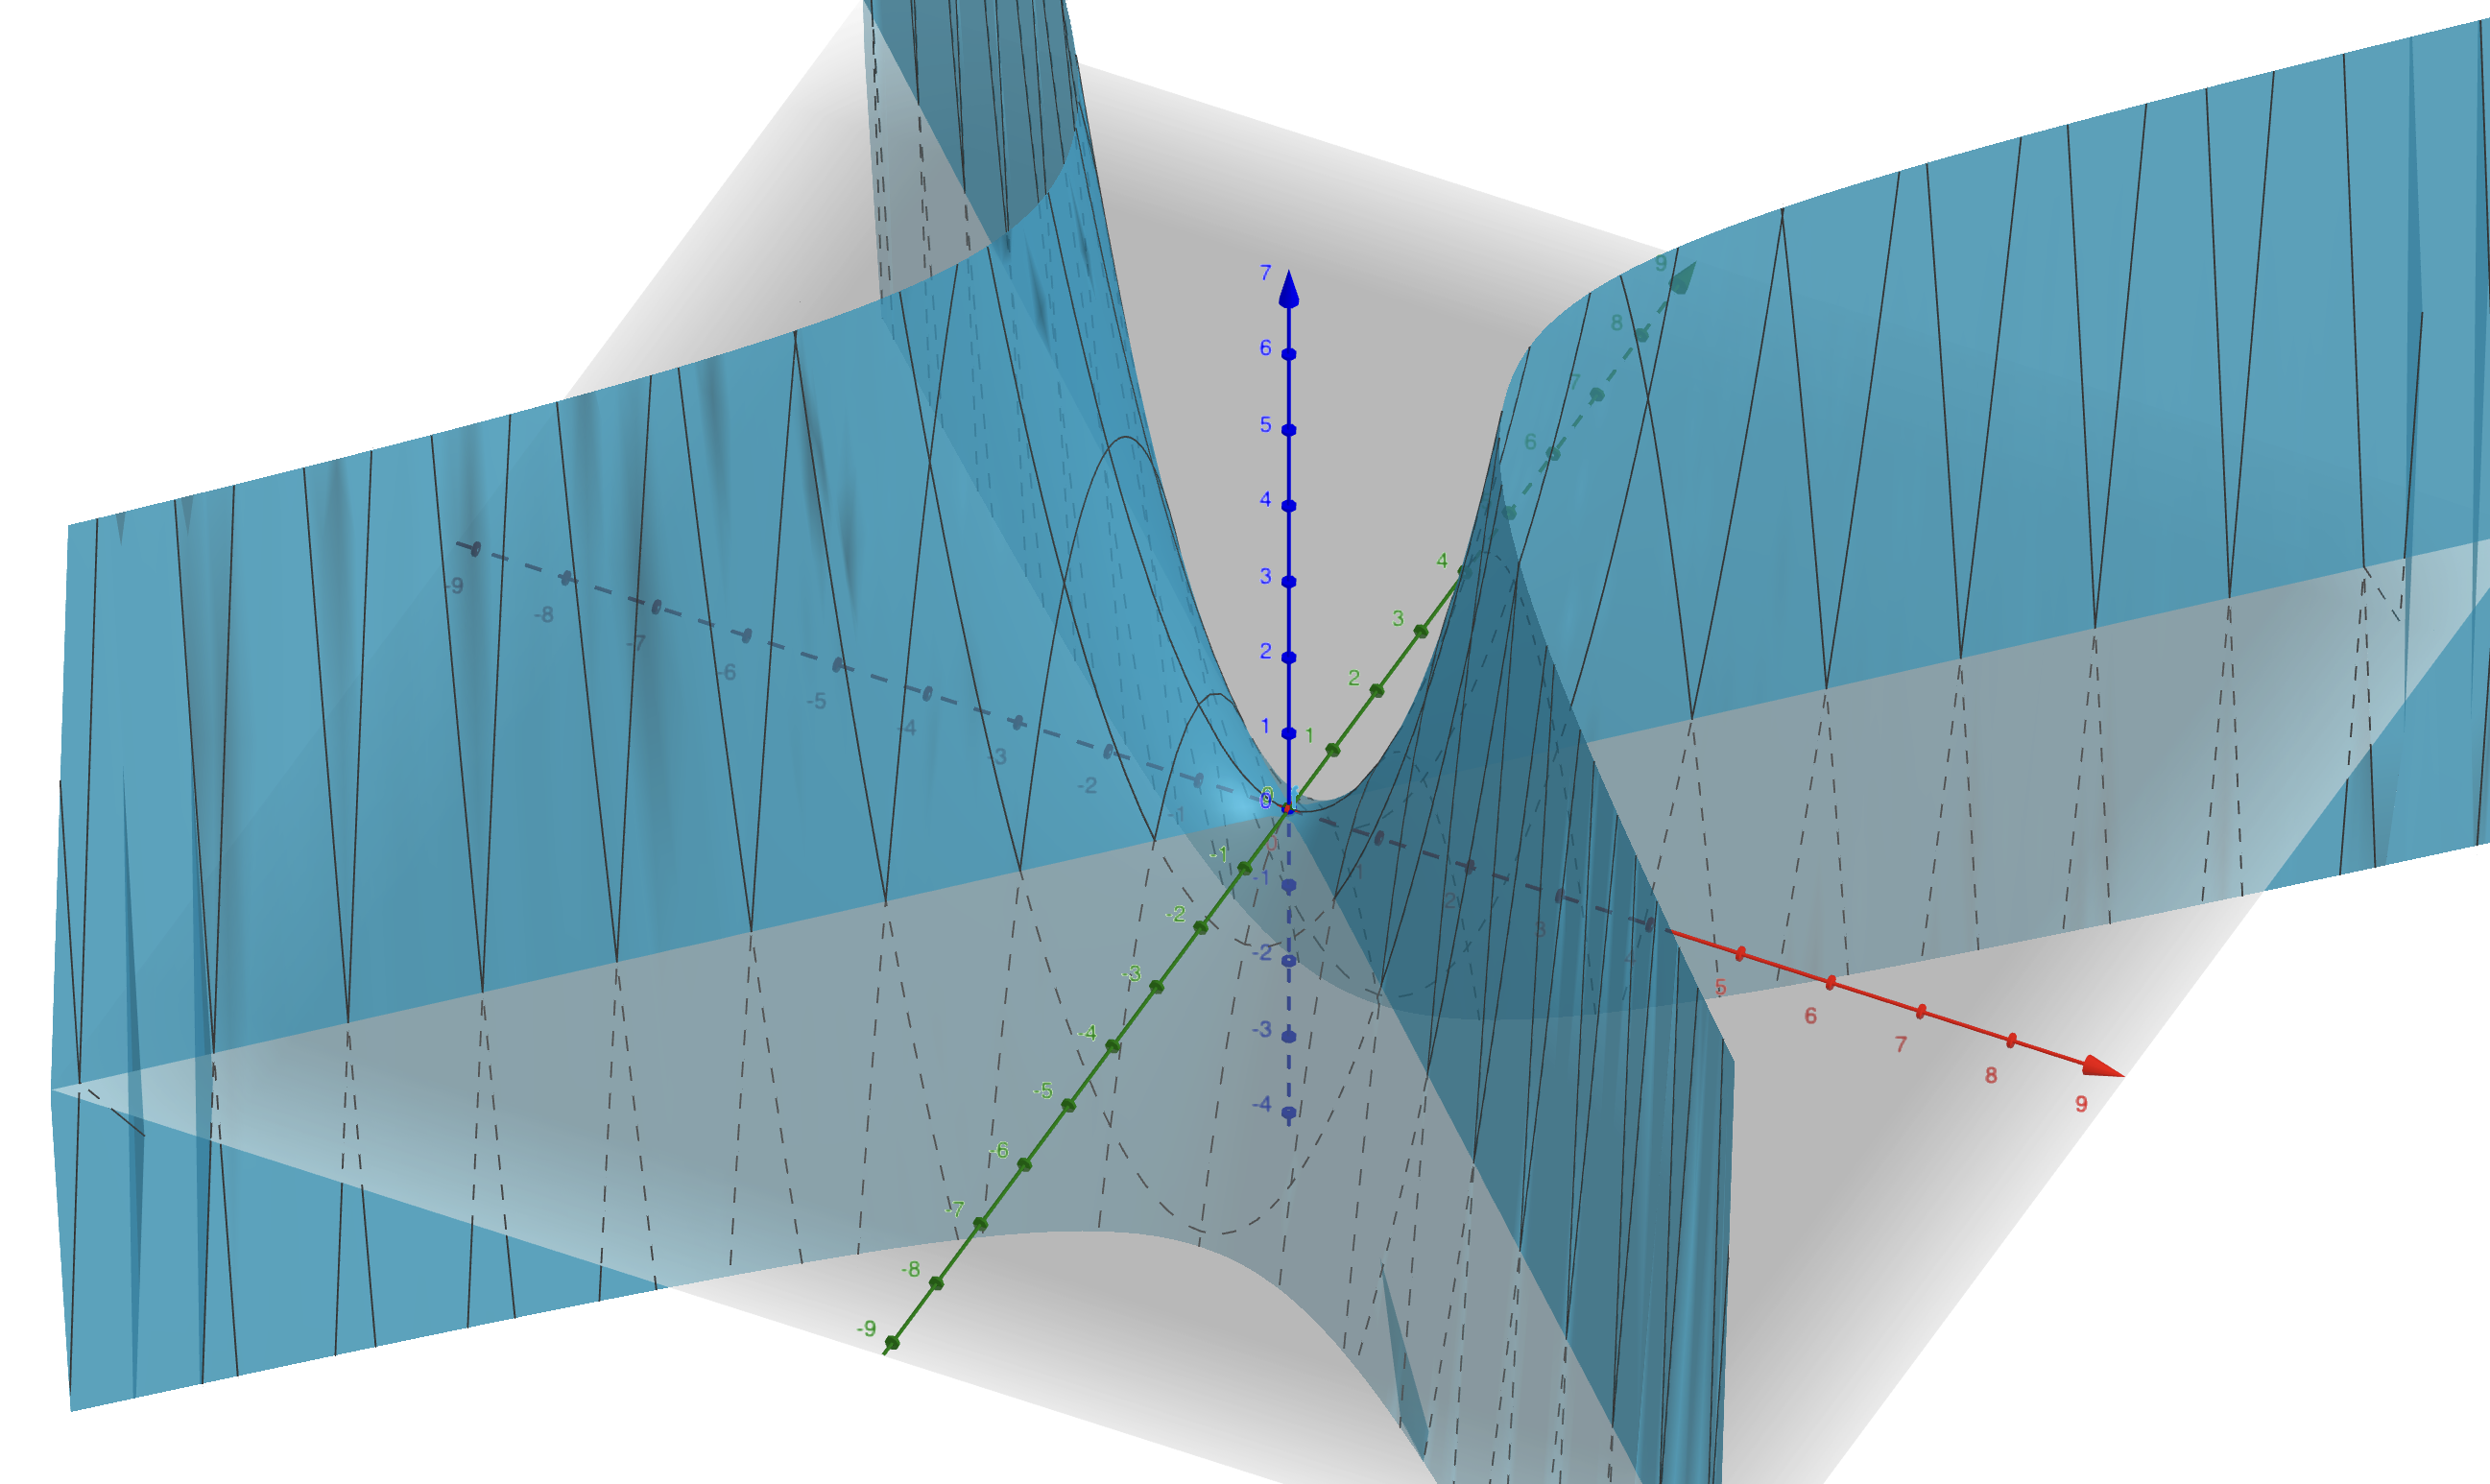
\includegraphics[scale=0.2]{images/Screen Shot 2022-10-26 at 02.39.56.png}
            \caption{$f(x,y)=x^2-y^2$}
        \end{figure}
    \end{itemize}
\end{itemize}

\begin{definition}
    Let $f:\R^2\longrightarrow \R$. A point $a$ is called a \underline{saddle point} if all partial derivatives $D_if(a)=0$ but $a$ is neither a maxima nor a minima.
\end{definition}

\begin{theorem*}[The Second Partial Derivative Test For Two variables]
    Let $f:\R^2\longrightarrow \R$ be of class $C^2$. Let 
    $$h=D_1D_1f(x)\cdot D_2D_2f(x)-(D_1D_2f(x))^2$$
    If $\nabla f(x)=\vec{0}$, then
    \begin{enumerate}
        \item If $h>0$ and $D_1D_1f(x)>0$, then  $x$ is a minima.
        \item If $h>0$ and $D_1D_1f(x)<0$, then  $x$ is a maxima.
        \item If $h<0$, then $x$ is a saddel point.
    \end{enumerate}
\end{theorem*}
\noindent \textbf{Example}:
\begin{itemize}
    \item Find all maxima and minima for $$f(x,y)=3x^2y-y^3-3x^2-3y^2$$
    First, solve the equation $$\nabla f(x)=\begin{bmatrix}
        D_1f(x,y)\\
        D_2f(x,y)
    \end{bmatrix}=\begin{bmatrix}
        6xy-6x\\
        3x^2-3y^2-6y
    \end{bmatrix}=\begin{bmatrix}
        0\\
        0
    \end{bmatrix}$$
    We get four points: $(0,0)$, $(0,-2)$, $(\sqrt{3},1)$, $(-\sqrt{3},1)$.
    $$D_1D_1f(x,y)=6y-6$$
    $$D_2D_1f(x,y)=6x$$
    $$D_2D_2f(x,y)=-6y-6$$
    \begin{figure}[H]
        \centering
        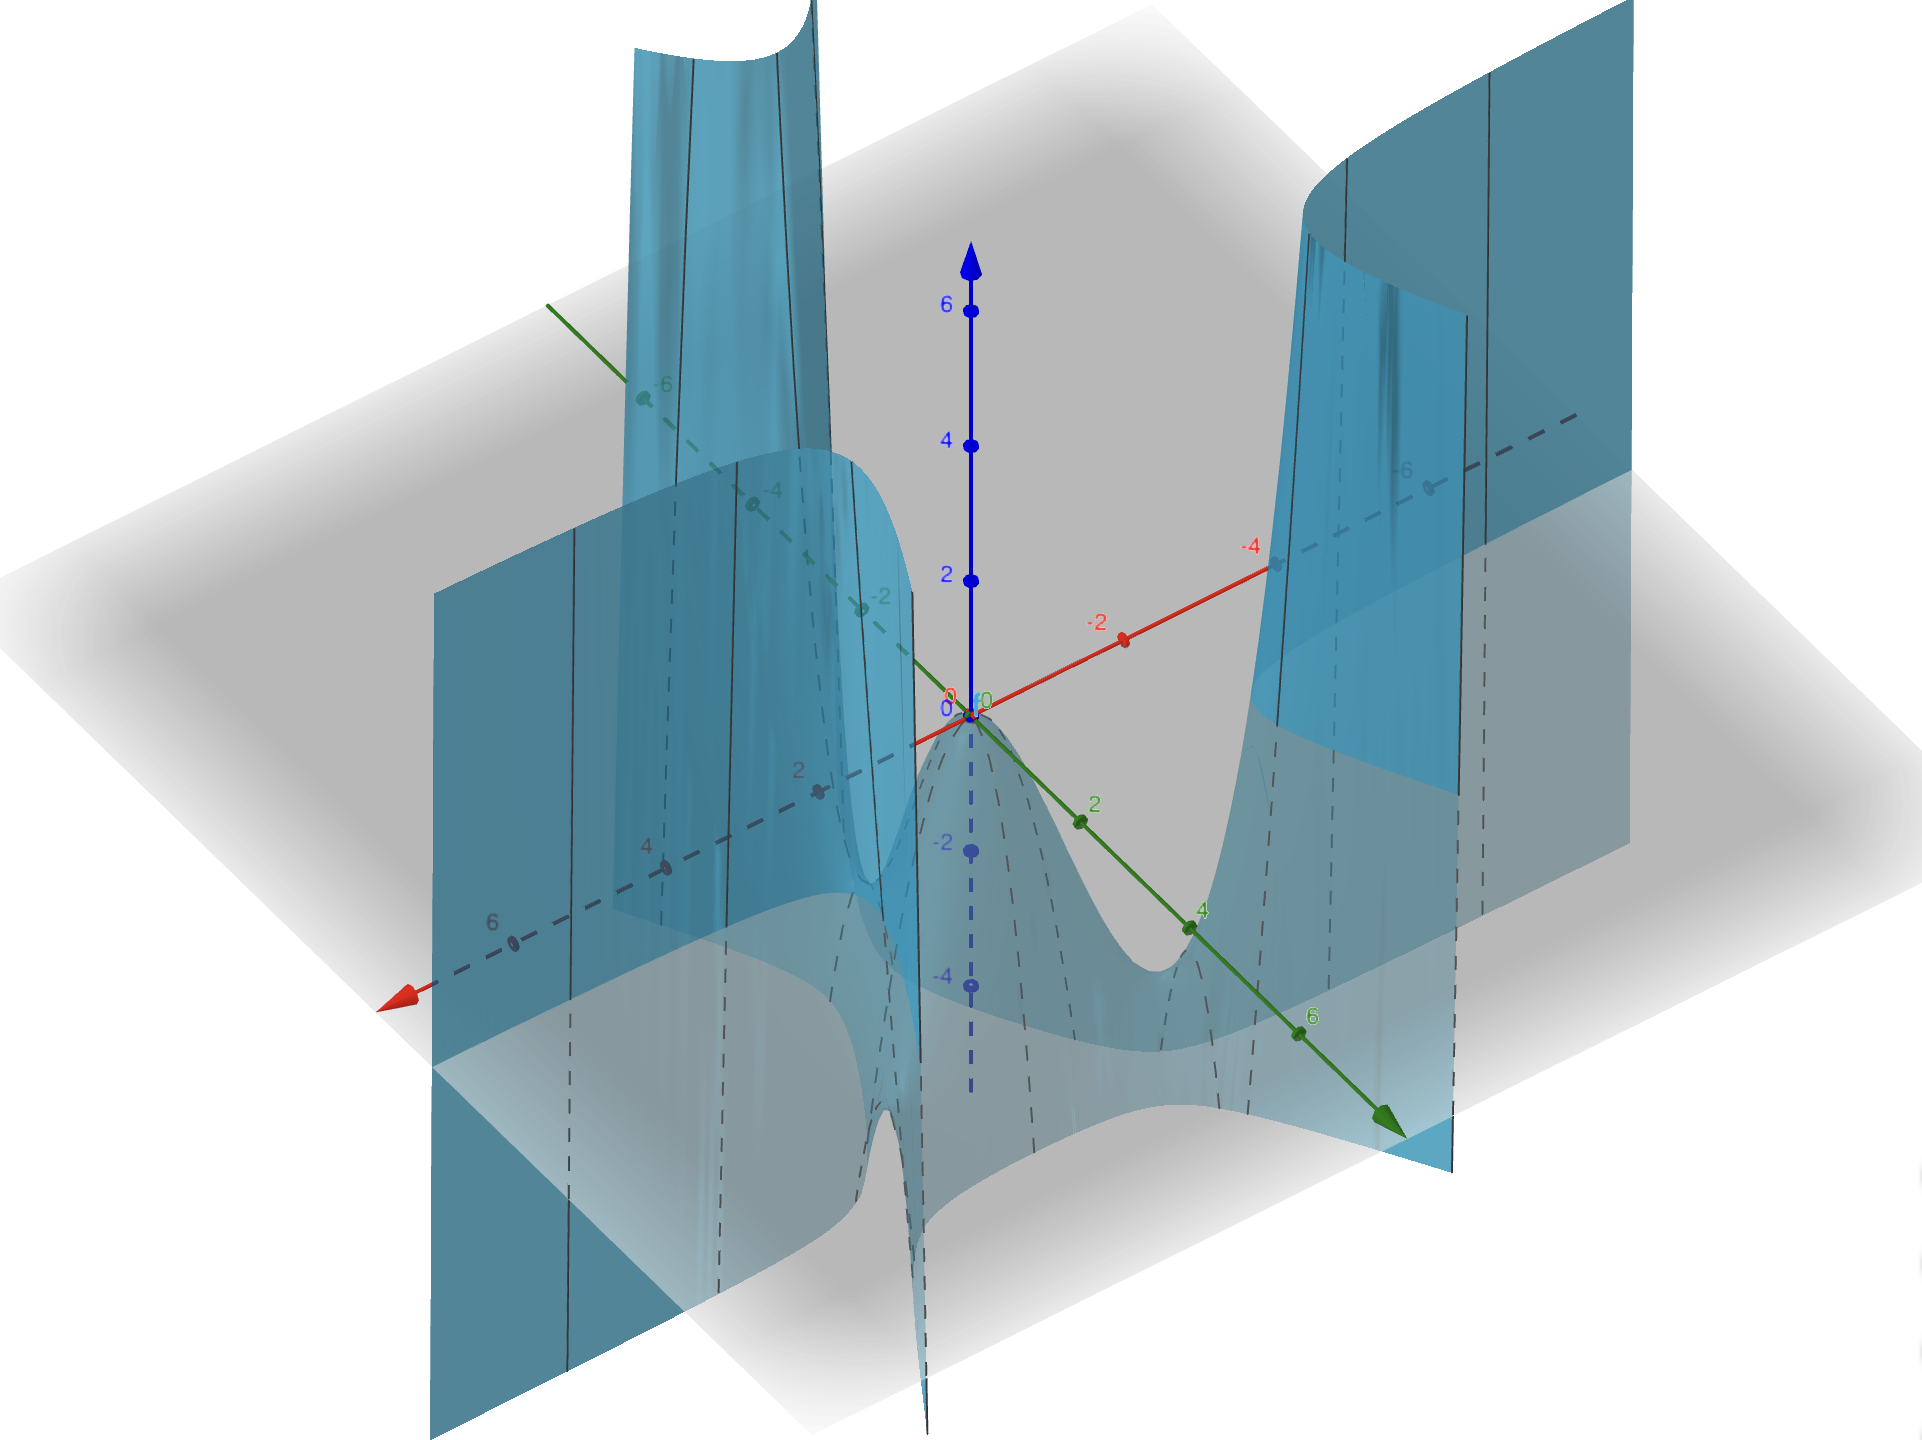
\includegraphics[scale=0.21]{images/Screen Shot 2022-10-26 at 03.53.45.png}
        \caption{$f(x,y)=3x^2y-y^3-3x^2-3y^2$}
    \end{figure}
    \begin{itemize}
        \item $(0,0)$: $h=(-6)(-6)-0^2>0 \Longrightarrow (0,0)$ is a maxima.
        \item $(0,-2)$: $h=(-18)(6)-0^2<0 \Longrightarrow (0,-2)$ is a saddle point.
        \item $(\sqrt{3},1)$: $h=0(-6)-108<0 \Longrightarrow (\sqrt{3},1)$ is a saddle point.
        \item $(-\sqrt{3},1)$: $h=0(-6)-108<0 \Longrightarrow (-\sqrt{3},1)$ is a saddle point.
    \end{itemize}
\end{itemize}
\noindent \textbf{Remark}:
\begin{itemize}
    \item In this case, $h=det(Hf)$.
    \item In order to generalize this criterion to $n$ variables, we need the following definitions.
\end{itemize}

\begin{definition}
    Let $A$ be a n by n matrix. We say $A$ is \underline{symmetric} if and only if $$A=A^T$$
\end{definition}
\noindent \textbf{Remark}:
\begin{itemize}
    \item The Hessian matrix $Hf$ is always symmetric.
\end{itemize}

\begin{definition}
    Let $A$ be a n by n symmetric matrix with real entries.
    \begin{enumerate}
        \item We say $A$ is \underline{positive-defined} if for all $x\in \R^n$
        $$x^TAx>0$$
        \item We say $A$ is \underline{negative-defined} if for all $x\in \R^n$
        $$x^TAx<0$$
        \item We say $A$ is \underline{indefined} if for all $x\in \R^n$
        $$x^TAx=0$$
    \end{enumerate}
\end{definition}

\begin{theorem*}
    Let $A=(a_{i,j})$ be a n by n symmetric matrix with real entries.
    \begin{enumerate}
        \item $A$ is positive-defined if and only if
        $$a_{1,1}>0, \quad \begin{vmatrix}
            a_{1,1} & a_{1,2}\\
            a_{2,1} & a_{2,2}
        \end{vmatrix}>0, \quad \begin{vmatrix}
            a_{1,1} & a_{1,2} & a_{1,3}\\
            a_{2,1} & a_{2,2} & a_{2,3}\\
            a_{3,1} & a_{3,2} & a_{3,3}
        \end{vmatrix}>0, \quad \cdots \quad det(A)>0$$
        \item $A$ is negative-defined if and only if
        $$a_{1,1}<0, \quad \begin{vmatrix}
            a_{1,1} & a_{1,2}\\
            a_{2,1} & a_{2,2}
        \end{vmatrix}>0, \quad \begin{vmatrix}
            a_{1,1} & a_{1,2} & a_{1,3}\\
            a_{2,1} & a_{2,2} & a_{2,3}\\
            a_{3,1} & a_{3,2} & a_{3,3}
        \end{vmatrix}<0, \quad \begin{vmatrix}
            a_{1,1} & a_{1,2} & a_{1,3} & a_{1,4}\\
            a_{2,1} & a_{2,2} & a_{2,3} & a_{2,4}\\
            a_{3,1} & a_{3,2} & a_{3,3} & a_{3,4}\\
            a_{4,1} & a_{4,2} & a_{4,3} & a_{4,4}
        \end{vmatrix}>0\cdots$$
    \end{enumerate}
\end{theorem*}

\begin{theorem*}[The Second Partial Derivative Test]
    Let $f:\R^n\longrightarrow \R$ be of class $C^2$.\\
    If $\nabla f(x)=\vec{0}$, then
    \begin{enumerate}
        \item If $Hf(x)$ is positive-defined, then  $x$ is a minima.
        \item If $Hf(x)$ is negative-defined, then  $x$ is a maxima.
        \item If $Hf(x)$ is indefined, then $x$ is not an extrema.
    \end{enumerate}
\end{theorem*}

\begin{definition}
    A \underline{contour line} (also isoline, isopleth, or isarithm) of a function of two variables is a curve along which the function has a constant value, so that the curve joins points of equal value.
\end{definition}
\noindent \textbf{Remark}:
\begin{itemize}
    \item The gradient of the function is always perpendicular to the contour lines.
    \begin{figure}[H]
        \centering
        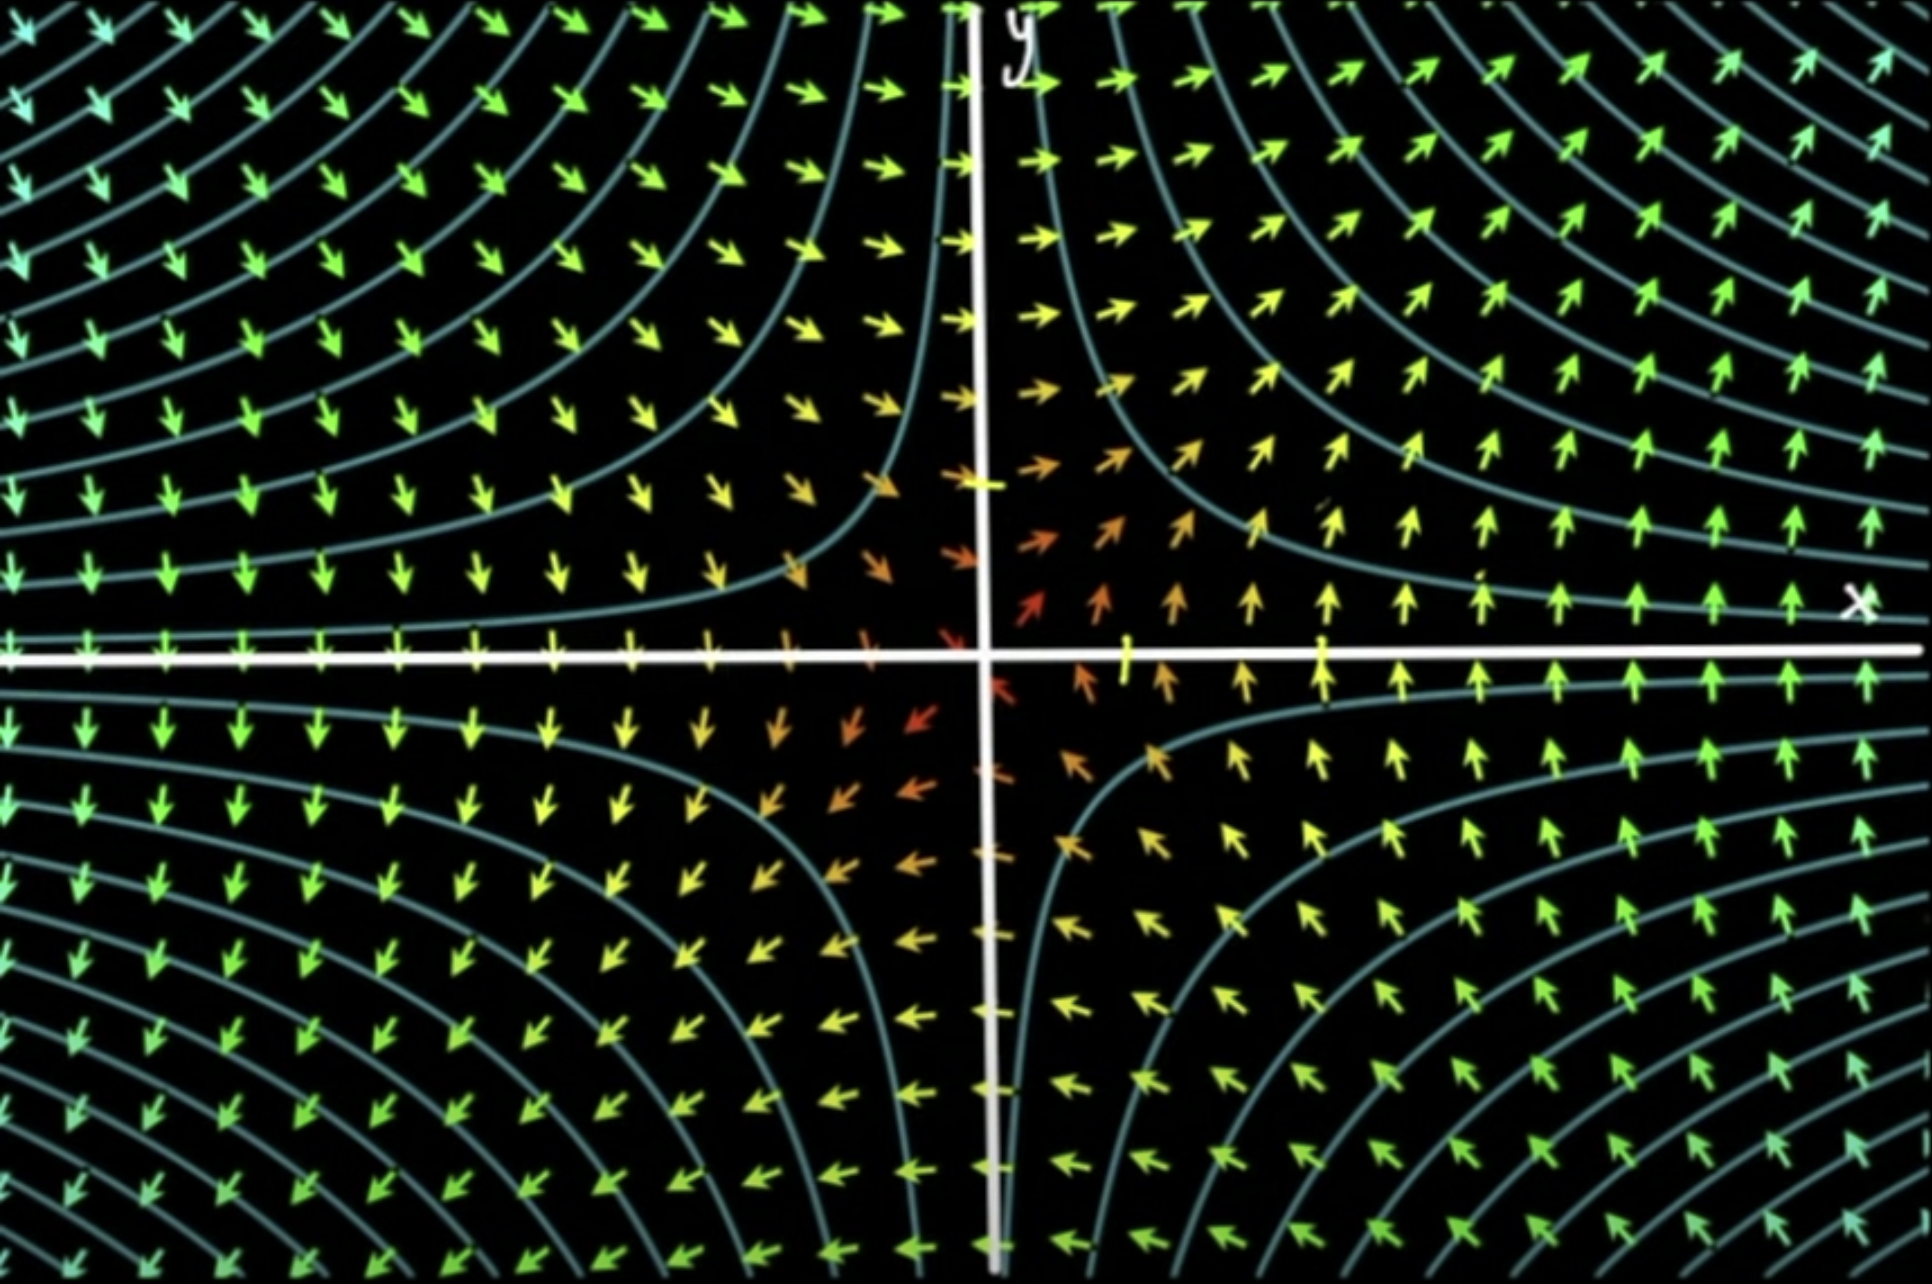
\includegraphics[scale=0.3]{images/Screen Shot 2022-10-26 at 13.04.34.png}
        \caption{Contour lines and gradient for $f(x,y)=xy$}
    \end{figure}
    \item When the lines are close together the magnitude of the gradient is large: the variation is steep.
    \item The idea of contour lines is very useful in real world applications like physics, geology,social science.
\end{itemize}

\begin{theorem}[Lagrange Multiplier]
    Given a function $f:A\subset \R^n\longrightarrow \R$, and constrains
    $$g_1(x_1,\cdots,x_n)=0,\cdots ,g_k(x_1,\cdots,x_n)=0$$
    We can solve the system of equations to get all critical points.
    \begin{equation}
        \begin{cases}
            \nabla f(x)=\sum_{i=1}^k \lambda_i \nabla g_i(x)\\
            g_1(x)=\cdots=g_k(x)=0
        \end{cases}
    \end{equation}
\end{theorem}
\noindent \textbf{Example}:
\begin{itemize}
    \item Find the maximum of $f(x,y)=x^2y$ given the constrain $g(x,y)=x^2+y^2-1=0$.\\
    \begin{figure}[H]
        \centering
        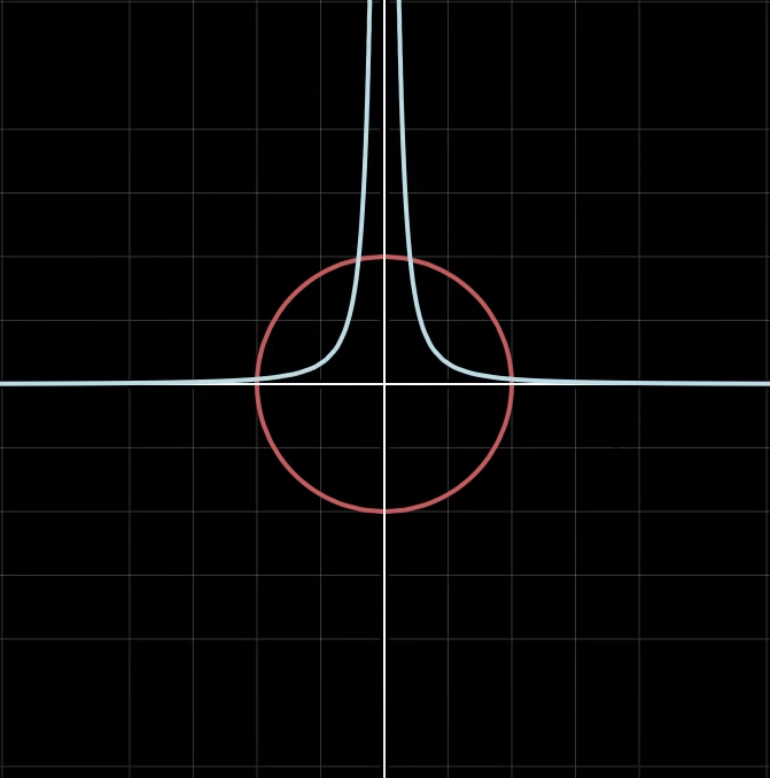
\includegraphics[scale=0.4]{images/Screen Shot 2022-10-26 at 14.31.58.png}
        \caption{One of the contour lines of $f$ and $g$.}
    \end{figure}
    
    As shown in the picture, the red circle represent the contour line of $g$ for $g(x)=0$. Our goal is to find the contour line of $f$ which is tangent to this red circle.
    We already know that the gradient is always perpendicular to the contour line. So the equation $$\nabla f(x)=\lambda \nabla g(x)$$
    gives us all the cases that one of the contour line of $f$ is tangent to one of the contour line of $g$. The equation $$g(x)=0$$
    constrain the contour line of $g$ to this red circle. So solving the system of equations 
    \begin{equation}
        \begin{cases}
            \nabla f(x)=\lambda \nabla g(x)\\
            g(x)=0
        \end{cases}
    \end{equation}
    will give us all the critical points. further, if we check all the value of these pointss, we can get the maximum and he minimum we want.
    $$\nabla f =\begin{bmatrix}
        D_1f\\
        D_2f
    \end{bmatrix}=\begin{bmatrix}
        2xy\\
        x^2
    \end{bmatrix}$$
    $$\nabla g =\begin{bmatrix}
        D_1g\\
        D_2g
    \end{bmatrix}=\begin{bmatrix}
        2x\\
        2y
    \end{bmatrix}$$
    Therefore, we need to solve 
    \begin{equation}
        \begin{cases}
            2xy=\lambda \cdot 2x\\
            x^2=\lambda\cdot 2y\\
            x^2+y^2=1
        \end{cases}
    \end{equation}
    We get four points: $(\sqrt{\frac{2}{3}},\sqrt{\frac{1}{3}})$, $(-\sqrt{\frac{2}{3}},\sqrt{\frac{1}{3}})$, $(\sqrt{\frac{2}{3}},-\sqrt{\frac{1}{3}})$, $(-\sqrt{\frac{2}{3}},-\sqrt{\frac{1}{3}})$\\
    Can check that the first point and the second point are both the maximum we want.
    \begin{figure}[H]
        \centering
        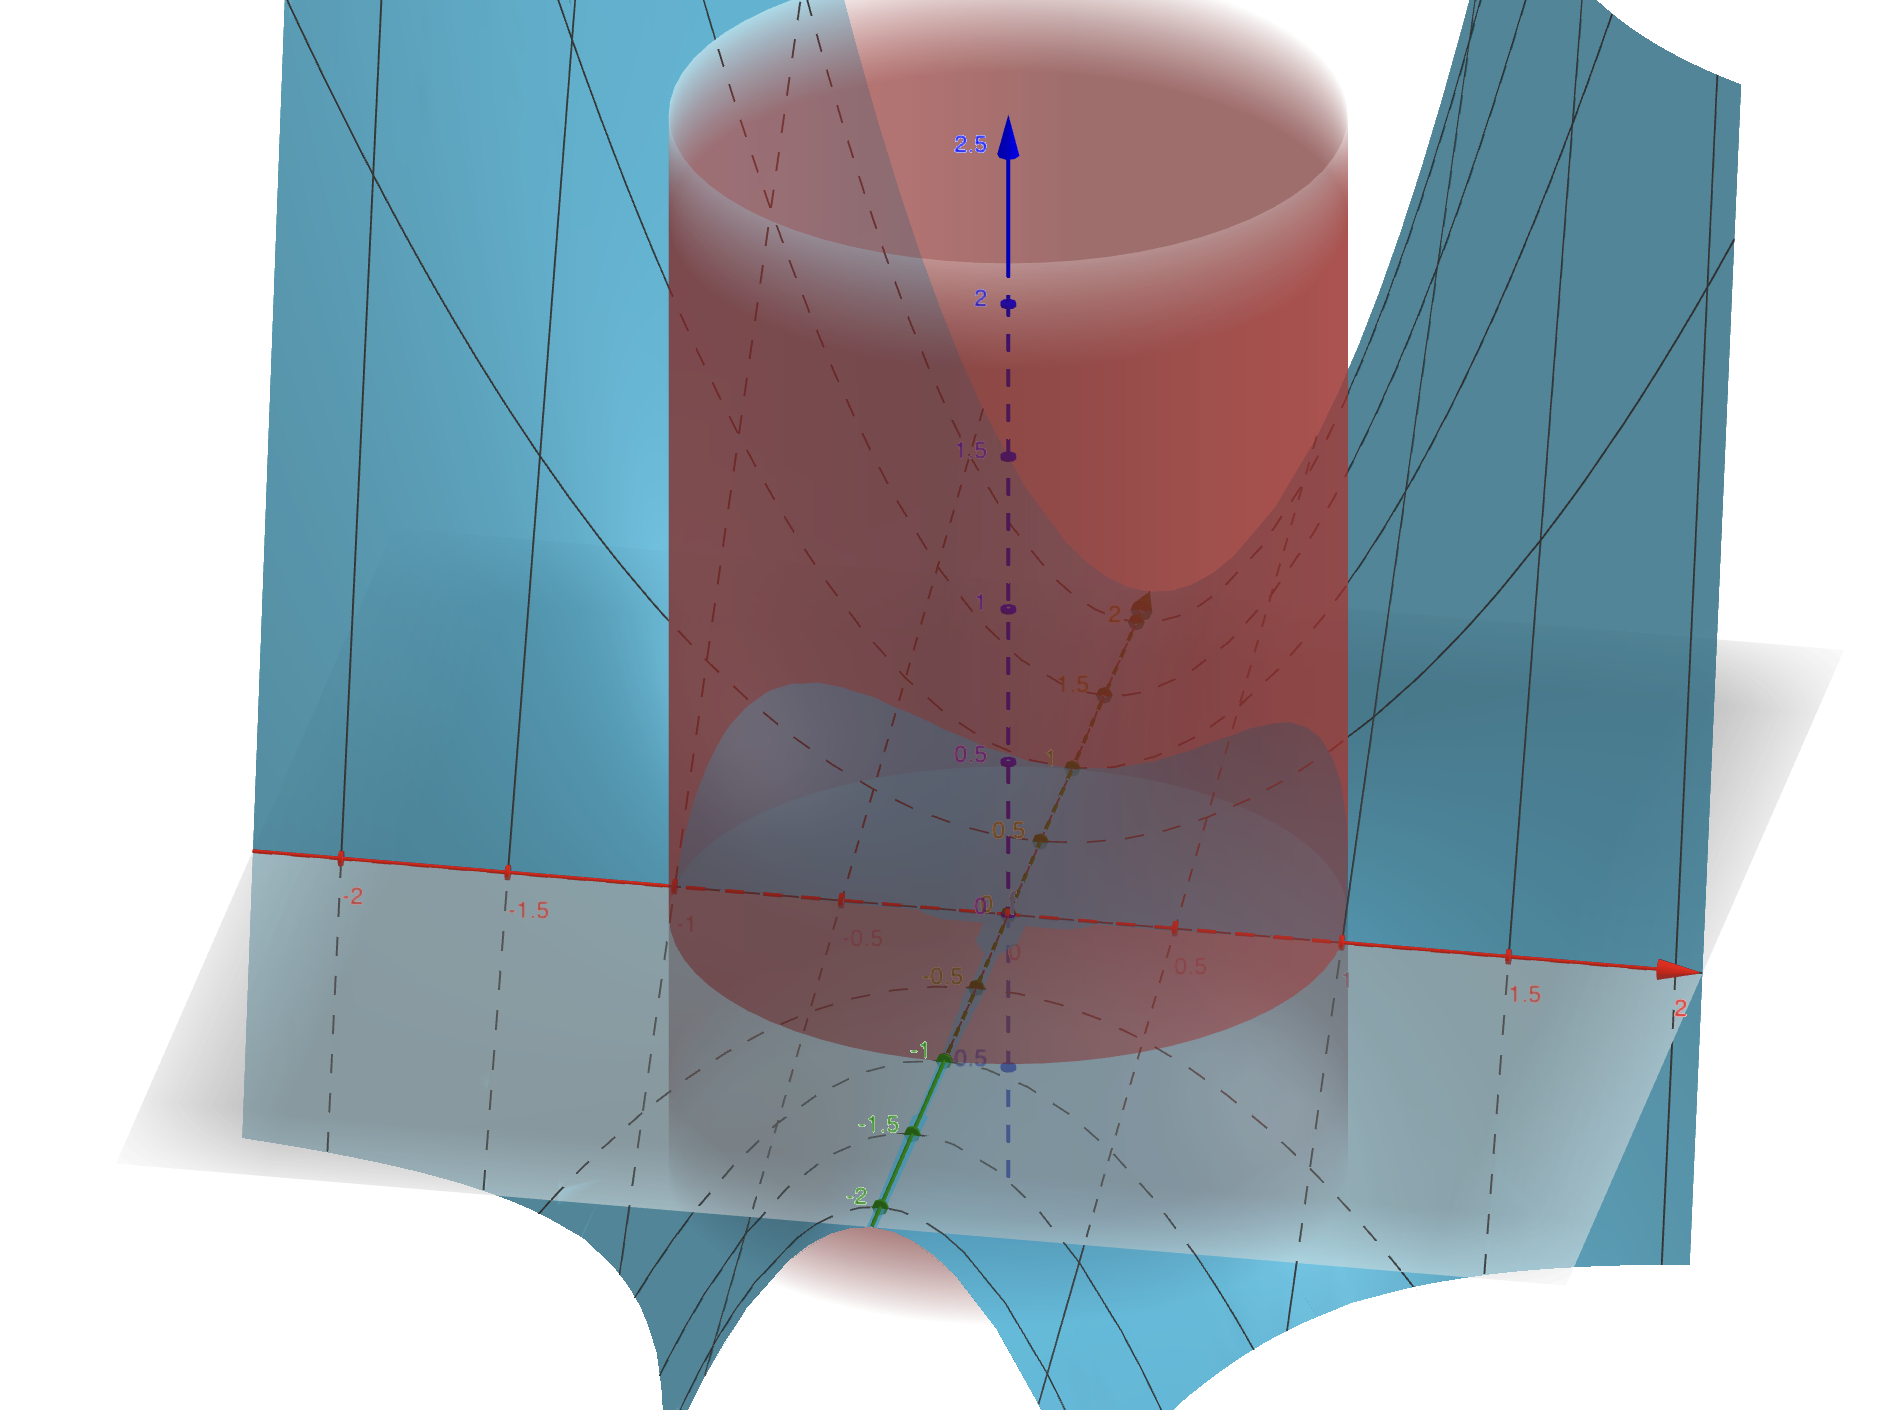
\includegraphics[scale=0.3]{images/Screen Shot 2022-10-26 at 15.13.16.png}
        \caption{$f(x,y)=x^2y$ and $x^2+y^2=1$}
    \end{figure}
\end{itemize}
\noindent \textbf{Remark}:
\begin{itemize}
    \item If the constrain is $g(x_1,\cdots,x_n)=(a_1,\cdots,a_m)$ for $(a_1,\cdots,a_m)\in \R^m$. Then this constrain can be viewed as 
    $$g_1(x_1,\cdots,x_n)=a_1,\cdots,g_m(x_1,\cdots,x_n)=a_m$$
\end{itemize}